\documentclass[12pt]{article}
\usepackage[latin1]{inputenc}
\usepackage{graphicx,subfigure}
\topmargin -1mm
\oddsidemargin -1mm
\evensidemargin -1mm
\textwidth 165mm
\textheight 220mm
\parskip 2mm
\parindent 3mm
%\pagestyle{empty}

\begin{document}

\begin{center}

{\Large \bf Documentation of the implementation of an algorithm to
  calculate thermodynamic equilibria in multi-component systems for
  flexible sets of conditions.}

\bigskip

Bo Sundman

\bigskip

Gif sur Yvette, France

\bigskip

DRAFT Version \today

\end{center}

%{\bf Keywords:} Computational Thermodynamics; Calphad; Equilibrium
%calculations; Modelling; Global minimization; Simulations;

\abstract{Thermodynamics is a central part in materials science.
Thermodynamic models provides a unique method to combine experimental
data and results from first principle calculations in databases.
These databases are essential to provide values of many different
thermodynamic properties in software tools for simulating materials
processes and to predict their final properties.

A well established algorithm to calculate thermodynamic
equilibria for multi-component systems using different kinds of
conditions and with many non-ideal solution phases modelled in
different ways is explained in detail.  In particular how to handle
phases with variable amount of atoms and how to handle different types
of conditions and changes of the set of stable phases during
iterations.

The algorithm can also be used to calculate properties outside the
equilibrium state as required for the simulation of phase
transitions.}

\bigskip

This is part of the documentation of the Open Calphad (OC) initiative.
There is also documentation available for the model package~\cite{gtp}
and there is ongoing work to develop and document the step/map/plot
procedures.  There is also development of an application software
interface called TQOC.  Finally there is a user guide to the command
oriented user interface to OC~\cite{OCui}.

The current release of the OC software and its documentation is
available at \cite{opencalphad} and the last update at~\cite{github}.

\newpage

\tableofcontents

\newpage

\section{Introduction}

The algorithm presented here was derived and explained in slightly
different forms by Gunnar Erikssom~\cite{75Eri}, Mats
Hillert~\cite{81Hil} and in the thesis by Bo Jansson~\cite{84Jan} and
in a paper by Leo Lukas~\cite{82Luk}.  These papers give the
theoretical background of the algorithm but they are very dense and
difficult to understand.  In a recent paper the algorithm and its
implementation is explained in more detail by Bo
Sundmanal.\cite{15Sun2}.  Some corrections and extentions comparated
to the published version are included in this documentation.

The implementation is done as part of the Open Calphad
initiative~\cite{15Sun1} to provide a free software for thermodynamic
calculations.  This software will provide a useful link between
experimental work, first principle calculations and applications like
simulatons of phase transformations and microstructures using phase
field methods.

\section{The thermodynamic model}

Phases in a thermodynamic system can be very different, examples are
gas, liquid, amorpheous and many different crystalline forms.  In any
system the Gibbs energy, $G$, is given at equilibrium by

\begin{equation}
G = \sum_{\alpha} \aleph^{\alpha} G_M^{\alpha}(T,P,Y) \label{eq:gmsum}
\end{equation}
where $\aleph^{\alpha}$ is the number of moles of formula units of the
phase $\alpha$ and $G_M^{\alpha}$ is the Gibbs energy per mole formula
unit of $\alpha$.  Each phase can be modelled differently but its
Gibbs energy depend on the temperature, pressure and its constitution,
here denoted by $T, P$ and $Y$.

Note that this definition of the molar Gibbs energy is different from
the normal

\begin{equation}
G_m = \frac{G}{N}\label{eq:molg1}
\end{equation}
where $N$ is the total number of moles of components.  But in this
paper $G_M$ will always be used according to the definition in
eq.~\ref{eq:gmsum}, using the formula unit explained in the next
section.

At equilibrium at constant $T, P$ and overall composition will be at a
minimum in the Gibbs energy.  For other conditions like volume,
chemical potential etc we can add Lagrangian constraints to obtain
the appropriate function to minimize.  Internal constraints, that the
sum of constituent fraction on each sublattice can also be handelled
by Lagarangian multipliers.

Each phase can be described with a different model but the
explanations in this paper will mainly concern phases modelled with
the compound energy formalism (CEF)~\cite{81Sun,01Hil}.  This include
as special gases ideal gases, substitutional regular soultions,
interstitial solutions, sublattice models etc. Some additional
explanations will be given for the ionic liquid model~\cite{84Hil}.

\subsection{The formula unit of a phase}

For a phase modelled with CEF we can have sublattices and the ratio
of these are deonoted $a_s$, where $s$ is the sublattice.  For example
the $\sigma$ phase has 5 sublattices with $a_s$ equal to 2, 4, 8, 8
and 8 sites.  Sites can be whole numbers or fractions but the
recommendation is to use the smallest integer values.  Thus a Laves
phase should be modelled (A,B)$_2$(A,B)$_1$ rather than
(A,B)$_{0.666667}$(A,B)$_{0.333333}$ as the number of decimal digits
may affect the mass balance as well as the Gibbs energy.

The constituent fraction for a phase $\alpha$ are denoted
$y_i^{\alpha}$.  For a phase with sublattices there will also be a
second index, $s$, $y_{is}^{\alpha}$ indicating the sublattice, as the
same species $i$ may be a constituent of several sublattices.  When
there is no possible confusion the phase and sublattice superscripts
are often omitted and a summation over $i$ will mean for all
constituents in all sublattices.

For ease of understanding we will from now on use indices A, B etc. to
denote components or elements and indices $i, j$ etc. to denote
constituents of a phase.  In many cases a constituent of a phase is
the same as an element but it can be a molecule or ion.  The meaning
of the term component is according the the Gibbs phase rule but a
component will often be the same as an element.

The number of moles of a component A per mole formula unit of the
phase, $M^{\alpha}_{\rm A}$ is calculated as
\begin{equation}
M_{\rm A}^{\alpha} = \sum_s a_s^{\alpha} \sum_i b_{{\rm A}i}
y_{is}^{\alpha} \label{eq:massfun}
\end{equation}
where $b_{{\rm A}i}$ is the stoichiometric factor of component A in
constituent $i$ and $y^{\alpha}_{is}$ is the fraction of constituent
$i$ in sublattice $s$ of phase $\alpha$.  As before $a_s$ is the
number of sites on sublattice $s$.  The sum of constituent fractions
on each sublattice is unity.

The total number of moles of components in a formula unit of the phase
is thus:
\begin{equation}
M^{\alpha} = \sum_{\rm A} M_{\rm A}^{\alpha} \label{eq:molesperfu}
\end{equation}
and the mole fraction is
\begin{equation}
x^{\alpha}_{\rm A} = \frac{M_{\rm A}^{\alpha}}{M^{\alpha}}
\end{equation}

The total number of moles of component A, $N_{\rm A}$, in a system
with several phases is
\begin{equation}
N_{\rm A} = \sum_{\alpha} \aleph^{\alpha} M_{\rm A}^{\alpha} \label{eq:mtot}
\end{equation}
where $\aleph^{\alpha}$ is the number of moles formula unit of the
phase $\alpha$.  The total number of moles of components, $N$, in the
system is

\begin{equation}
N = \sum_{\rm A} N_{\rm A} =
\sum_{\rm A} \sum_{\alpha} \aleph^{\alpha} M_{\rm A}^{\alpha}
\end{equation}
and the mole fraction of A in the whole system is
\begin{equation}
x_{\rm A} = \frac{N_{\rm A}}{N}
\end{equation}

We have to be careful to distinguish between $N, \aleph, M, x, y$ and
other composition related variables.

\subsection{Differentials}

The differential of $M^{\alpha}_{\rm A}$ is

\begin{equation}
dM^{\alpha}_{\rm A} = \sum_s \sum_i
\left(\frac{\partial M_{\rm A}^{\alpha}}{\partial y_{is}^{\alpha}}
\right)_{y_{j\ne i}} dy_{is}^{\alpha} \label{eq:diffm1}
\end{equation}
where each partial derivative of $M^{\alpha}_{\rm A}$ is

\begin{equation}
\left(\frac{\partial M_{\rm A}^{\alpha}}{\partial y_{is}}
\right)_{y_{j\ne i}} = a_s^{\alpha} b_{{\rm A}i}
\end{equation}

Most of these derivatives will be zero as $M_{\rm A}$ often depends on
a single or just a few $y_{is}$.  But we can have molecules with
several atoms as constituents and also vacancies in a sublattice and
the number of moles of components per formula unt of the phase is
often not fixed.

For the ionic liquid model the situation is different as the number of
sites for cations and anions depend on the average charge on the other
sublattice.  That will be discussed in the context of that model, It
does not affect the general procedure for the minimization of the
Gibbs energy described here.

\subsection{Examples}

Understanding the meaning of formula unit is essential to the
algorithm so a few examples will be given.

\subsubsection{A gas phase with H and O}

In a gas with the molecules (H$_2$, O$_2$, H$_2$O) the moles formula
unit of the components H and O and the total number of moles in a
formula unit, $M$, are:

\begin{eqnarray*}
M_{\rm H} &=& 2y_{\rm H_2} + 2y_{\rm H_2O}\\
M_{\rm O} &=& 2y_{\rm O_2} + y_{\rm H_2O}\\
M &=& 2y_{\rm H_2} + 2y_{\rm O_2} + 3y_{\rm H_2O}
\end{eqnarray*}

The number of moles of atoms per formula unit of this gas can thus
very between 2 and 3.  The mole fractions are:

\begin{eqnarray*}
x_{\rm H} = \frac{M_{\rm H}}{M} &=& \frac{2y_{\rm H_2} + 2y_{\rm H_2O}}
{2y_{\rm H_2} + 2y_{\rm O_2} + 3y_{\rm H_2O}}\\
x_{\rm O} = \frac{M_{\rm O}}{M} &=& \frac{2y_{\rm O_2} + y_{\rm H_2O}}
{2y_{\rm H_2} + 2y_{\rm O_2} + 3y_{\rm H_2O}}
\end{eqnarray*}

\subsubsection{A crystalline phase with substitutional and interstitial
constituents}

An interstitial solution of C and N in the bcc phase in a steel with
Cr is modelled (Cr, Fe)$_1$(C, N, Va)$_3$, where Va denotes a vacancy
or vacant site.  The moles formula units of the elements are:

\begin{eqnarray*}
M_{\rm C} &=& 3y_{\rm C,2}\\
M_{\rm Cr} &=& y_{\rm Cr,1}\\
M_{\rm Fe} &=& y_{\rm Fe,1}\\
M_{\rm N} &=& 3y_{\rm N,2}\\
M &=& 1+3y_{\rm C,2}+3y_{\rm N,2}
\end{eqnarray*}

We use a comma between the constituent and the sublattice when they
are explicit.  If there are only two sublattices one frequently use
one or two primes, $y'_{\rm Cr}$ and $y''_{\rm C}$ to indicate the
sublattice but with more than two sublattices that become cumbersome.
The number of moles of atoms per formula unit of the bcc phase can
thus very between 1 and 4.  He mole fractions are:

\begin{eqnarray*}
x_{\rm C} &=& \frac{3y_{\rm C,2}}{1+3y_{\rm C,2}+3y_{\rm N,2}}\\
x_{\rm Cr} &=& \frac{y_{\rm Cr,1}}{1+3y_{\rm C,2}+3y_{\rm N,2}}\\
x_{\rm Fe} &=& \frac{y_{\rm Fe,1}}{1+3y_{\rm C,2}+3y_{\rm N,2}}\\
x_{\rm N} &=& \frac{3y_{\rm N,2}}{1+3y_{\rm C,2}+3y_{\rm N,2}}\\
\end{eqnarray*}

\subsubsection{A crystalline phase with long range ordering}

Finally for a $\sigma$ phase in the Cr, Fe, Mo and Ni system modelled
with only 3 sublattices and with restricted solublities, (Cr, Fe,
Ni)$_{10}$(Cr, Mo)$_4$(Cr, Fe, Mo, Ni)$_{16}$, the moles formula units
are

\begin{eqnarray*}
M_{\rm Cr} &=& 10y_{\rm Cr,1} + 4y_{\rm Cr,2} + 16y_{\rm Cr,3}\\
M_{\rm Fe} &=& 10y_{\rm Fe,1}+16y_{\rm Fe,3}\\
M_{\rm Mo} &=& 4y_{\rm Mo,2}+16y_{\rm Mo,3}\\
M_{\rm Ni} &=& 10y_{\rm Ni,1}+16y_{\rm Ni,3}\\
M &=& 30
\end{eqnarray*}

The number of moles per formula unit is constant and equal to 30.  The
mole fractions are

\begin{eqnarray*}
x_{\rm Cr} &=& \frac{10y_{\rm Cr,1} + 4y_{\rm Cr,2} + 16y_{\rm Cr,3}}{30}\\
x_{\rm Fe} &=& \frac{10y_{\rm Fe,1}+16y_{\rm Fe,3}}{30}\\
x_{\rm Mo} &=& \frac{4y_{\rm Mo,2}+16y_{\rm Mo,3}}{30}\\
x_{\rm Ni} &=& \frac{10y_{\rm Ni,1}+16y_{\rm Ni,3}}{30}
\end{eqnarray*}

The reason for this somewhat lenghty explanation is it is very common
to make misstakes, or be uncertain using different kinds of variables
for the amount of material in a system or phase.

\subsection{End-members of models}

An important concept when modelling with CEF is the {\em end-member}
which for a crystalline phase specifies one constituent in each
sublattice of the phase.  A phase can consist o a single end-member
and for the gas phase each molecule is an end-member.  In the bcc
phase example above we have 6 end-members which can be denoted:
(Cr:C), (Cr:N), (Cr:Va), (Fe:C), (Fe:N) and (Fe:Va).  In the $\sigma$
phase example there are 16 end-members, for example (Fe:Cr:Cr),
(Fe:Cr:Fe), (Fe:Cr:Mo), (Fe:Cr:Ni) etc.  Note that in most cases
end-members represent compounds with several elements.

\section{The Gibbs energy}

The Gibbs energy, $G$ is an extensive property and can be subdivided
in may different way.  One well known formula relates the Gibbs energy
to the chemical potentials, $\mu_{\rm A}$, and the number of moles,
$N_{\rm A}$ of the components:

\begin{equation}
G = \sum_{\rm A} N_{\rm A} \mu_{\rm A} \label{eq:gsummu}
\end{equation}

The definition of the chemical potentials is

\begin{equation}
\mu_{\rm A}=\left(\frac{\partial G}{\partial N_{\rm A}}
\right)_{T,P,N_{\rm B\ne A}} \label{eq:mudef}
\end{equation}

If a phase has a fixed composition it has only a Gibbs energy and we
cannot calculate the individual chemical potentials of the components
for this phase alone.  But if we can vary the fraction of constituents
in one or more sublattices it is possible to calculate some relations
between chemical potentials as will be discussed below in the context
of eq.~\ref{eq:cmu}.

We have already introduced a different definition of the molar Gibbs
energy for each phase which is related to the formula unit of the
phase defined by structure of the phase as described above.  Using
eq.~\ref{eq:massfun} the molar Gibbs energy for a formula unit,
$G_M^{\alpha}$ and for one mole of components, $G_m^{\alpha}$, for a
phase $\alpha$ are equal to:

\begin{eqnarray}
G_M^{\alpha} &=& \sum_{\rm A} M_{\rm A}^{\alpha} \mu_{\rm A}\\
G_m^{\alpha} &=& \sum_{\rm A} x_{\rm A}^{\alpha} \mu_{\rm A}
\end{eqnarray}

So it is important to know what kind of ``molar'' quantity we use.

\subsection{The differential of the Gibbs energy}

The differential of the Gibbs energy is

\begin{equation}
dG = -SdT+VdP+\sum_{\rm A}\mu_{\rm A}dN_{\rm A} \label{eq:dg1}
\end{equation}
and at equilibrium in a closed system $dG=0$.  If we have several
stable phases

\begin{eqnarray}
dG &=& \sum_{\alpha}(\aleph^{\alpha}dG_M^{\alpha}+G_M^{\alpha}d\aleph^{\alpha})
\end{eqnarray}
where $dG_M^{\alpha}$ for each phase can, using the molar Gibbs energy
per formula unit, be expressed as differences of the independent
variables $T, P$ and $M_{\rm A}$ or the dependent $y^{\alpha}_{is}$:

\begin{eqnarray}
dG_M^{\alpha} &=& -S_M^{\alpha}dT+V_M^{\alpha}dP+
\sum_{\rm A}\mu_{\rm A}dM^{\alpha}_{\rm A} \nonumber\\&=&
-S_M^{\alpha}dT+V_M^{\alpha}dP+
\sum_{\rm A}\mu_{\rm A}\sum_s \sum_i
\left(\frac{\partial M^{\alpha}_{\rm A}}{\partial y^{\alpha}_{is}}
\right)_{T,P,y_{j\ne i}}
dy^{\alpha}_{is} \label{eq:dgmfu}
\end{eqnarray}

\subsection{The partial Gibbs energy with for an end-member}

For a phase with sublattices it is not always possible to calculate
directly the chemical potentials for the components but we can always
calculate the partial Gibbs energies of the end-members, $I$, of the
model.  An end-member specifies one constituent in each sublattice:

\begin{equation}
G_I=G_M + \sum_{s}\left(\frac{\partial G_M}{\partial y_{is\in I}}
\right)_{T,P,y_{j\ne i}}
- \sum_s \sum_{j} y_{js}\left(\frac{\partial G_M}{\partial y_{js}}
\right)_{T,P,y_{k\ne j}} \label{eq:mufory}
\end{equation}
where the first summation is for the constituents $i$ specified by the
end-member $I$ for each sublattice $s$.  The second double summation is
for all constituents $j$.  For a phase with fixed composition $G_I = G_M$.

In the example for the bcc interstitial solution (Fe, Cr)$_1$(C, N,
Va)$_3$ above it is not possible to express directly the partial Gibbs
energy for C in the model.  However, we have the end-members (Fe:Va)
and (Fe:C) and we can calculate these two partials from the model:

\begin{eqnarray}
G_{\rm Fe:Va}&=&G_M + \left(\frac{\partial G_M}{\partial y_{\rm Fe,1}}
\right)_{T,P,y_{j\ne {\rm Fe}}} +
\left(\frac{\partial G_M}{\partial y_{\rm Va,2}}
\right)_{T,P,y_{j\ne {\rm Va}}}
- \sum_s \sum_{j} y_{js}\left(\frac{\partial G_M}{\partial y_{js}}
\right)_{T,P,y_{k\ne j}} \nonumber\\&&\\
G_{\rm Fe:C}&=&G_M + \left(\frac{\partial G_M}{\partial y_{\rm Fe,1}}
\right)_{T,P,y_{j\ne {\rm Fe}}} +
\left(\frac{\partial G_M}{\partial y_{\rm C,2}}
\right)_{T,P,y_{j\ne {\rm C}}}
- \sum_s \sum_{j} y_{js}\left(\frac{\partial G_M}{\partial y_{js}}
\right)_{T,P,y_{k\ne j}} \nonumber\\&&
\end{eqnarray}

At equilibrium the partial Gibbs energies of the end-members are
related to the chemical potentials of the components as

\begin{eqnarray*}
G_{\rm FeVa_3} = G_{\rm Fe:Va} = G_{\rm Fe} &=& \mu_{\rm Fe}\\
G_{\rm FeC_3} = G_{\rm Fe:C} = G_{\rm Fe} + 3G_{\rm C} &=&
\mu_{\rm Fe} + 3\mu_{\rm C}
\end{eqnarray*}
as the chemical potential of Va, $\mu_{\rm Va}=0$ at equilibrium.  We
can rearrange to obtain the chemical potential of C:

\begin{eqnarray}
\mu_{\rm C} = G_{\rm C} = \frac{1}{3}(G_{\rm Fe:C}-G_{\rm Fe:Va}) &=&
\frac{1}{3}\left[\left(\frac{\partial G_M}{\partial y_{\rm C,2}}
\right)_{T,P,y_{\rm Va}} -
\left(\frac{\partial G_M}{\partial y_{\rm Va,2}}
\right)_{T,P,y_{\rm C}}\right] \label{eq:cmu}
\end{eqnarray}

As can be seen by the last part of eq.~\ref{eq:cmu} it is independent
of the constituent in the first sublattice so it does not matter if we
had chosen the end-members (Cr:C) and (Cr:Va).  At equilibrium the
difference will be the same.

Even of there is no Cr so Fe is alone on its sublattice we can obtain
the chemical potentials of both Fe and C because the fraction of C can
vary.

But for some CEF models it is not possible to combine the end-members
in such a way that one can extract the chemical potentials of the
elements, in the model for for the $\sigma$ phase above we cannot
obtain the individual chemical potentials of the elements from the
model.  But the method described below to calculate the equilibrium
can be applied also for such phases.

%\begin{eqnarray*}
%\end{eqnarray*}

\subsection{The Gibbs-Duhem relation}

In eq.~\ref{eq:dg1} there is no differential of the chemical
potentials because the Gibbs-Duhem relation for each phase is:

\begin{equation}
\sum_{\rm A}d\mu_{\rm A} M^{\alpha}_{\rm A}+S_M^{\alpha}dT+V_M^{\alpha}dP =0
\end{equation}
which must be valid at equilibrium.

\section{Minimization with constraints}

To minimize a function with constraints we apply a Lagarangian
equation where each equality constraints has a multiplier.  When the
constraint is obeyed the minimim of the Lagrangian is the same as the
origibal function.  The multipliers can be used to find the method to
vary the variables to fulfill the constraints.

\subsection{The constraints}

The variables in the Gibbs energy expression have several constraints.
The first is that the sum of the site fractions on each sublattice is
unity:

\begin{equation}
g^{\alpha}_s = 1 - \sum_i y^{\alpha}_{is} = 0
\end{equation}

For phases with ions the net charge must be zero and an external
charge balance constraint must be added:

\begin{equation}
Q^{\alpha} = \sum_s a_s \sum_i \nu_i y^{\alpha}_{is} = 0 \label{eq:qsum}
\end{equation}

\noindent
where $\nu_i$ is the charge on constituent $i$.

The total Gibbs energy for a system, $G$, is given by
eq.~\ref{eq:gmsum}.  The number of formula units of a phase $\alpha$,
$\aleph^{\alpha}$, must be equal to or larger than zero for a stable
phase.  If it becomes negative during iterations it will be removed
from the stable set of phases.

For a closed system we have the constraint on the amount of components

\begin{equation}
f_{\rm A}={\tilde N}_{\rm A}-N_{\rm A}={\tilde N}_{\rm
A}-\sum_{\alpha}\aleph^{\alpha}M^{\alpha}_{\rm A}=0
\end{equation}

\noindent
where ${\tilde N}_{\rm A}$ is the prescribed amount of component A.
For a phase modelled (A,B)$_{0.75}$(A,B)$_{0.25}$ the value of
$\aleph^{\alpha}$ is 4 times larger compared to the case that the
phase had been modelled (A,B)$_3$(A,B)$_1$.  Both models are allowed
and the thermodynamic parameters in the second case must be 4 times
larger than those in the first.

\subsection{The Lagrangian equation}

To minimize the Gibbs energy of a system with constraints we can use a
Lagrangian equation as:

\begin{equation}
L = G + \sum_{\rm A} f_{\rm A} \mu_{\rm A} +
\sum_{\alpha} \eta_s^{\alpha} g_{s}^{\alpha} +
\sum_{\alpha} \lambda^{\alpha} Q^{\alpha} +
\sum_{\psi} \gamma^{\psi} \aleph^{\psi}
\end{equation}

\noindent
where $\mu_{\rm A}, \eta_{s}^{\alpha}, \lambda^{\alpha}$ are
multipliers for all phases and $\gamma^{\psi}$ are multipliers for all
phases $\psi$ that are unstable with $\aleph^{\psi}=0$.  The
important property of this Lagrantian is that it will have the same
extremum points as the Gibbs energy $G$ when the constraints are
fullfilled.  From now on it will rarely be indicated which variables
are kept constant at the partial derivatives, the reader is expected
to understand this from the text.

\subsection{The derivative of the Lagrangian with respect to phase amounts}

For the partial derivative of $L$ with respect to the amount of a
stable phase $\alpha$ we get:

\begin{equation}
\frac{\partial L}{\partial \aleph^{\alpha}} = G^{\alpha}_M -
\sum_{\rm A} f_{\rm A} M^{\alpha}_{\rm A} = 0
\end{equation}
and from this equation we can understand that the Lagrangian
multiplier $f_{\rm A} = \mu_{\rm A}$, i.e. the chemical potential of
component A.  For a rigorous proof see~\cite{81Hil}.

For an unstable phase $\psi$ which is not included in the stable
phase set we can calculate the derivative:

\begin{equation}
\frac{\partial L}{\partial \aleph^{\psi}} = G^{\psi}_M -
\sum_i \mu_i M^{\psi_i} + \gamma^{\psi} = 0 \label{eq:dgm1}
\end{equation}

This means that the driving force, $\gamma^{\psi}$, for an unstable
phase will be calculated as part of the minimization.  An unstable
phase may become stable during the iterations for the equilibrium and
that is indicated by $\gamma^{\psi}$ becomming positive.

On the other hand, if $\aleph^{\alpha}$ for a stable phase $\alpha$
becomes negative it means this phase has become unstable and should be
removed from the stable set.  In both cases we must change the set of
stable phases as will be discussed in section~\ref{sc:changeps}.

\subsection{The derivative of the Lagrangian with respect to
constituent fractions}

The partial derivative of $L$ with respect to a constituent fraction
$y^{\alpha}_{is}$, keeping all other variables constant, we get:

\begin{equation}
\frac{\partial L}{\partial y^{\alpha}_{is}} =
\aleph^{\alpha}\frac{\partial G_M^{\alpha}}{\partial y^{\alpha}_{is}}
- \aleph^{\alpha}\sum_{\rm A} \mu_{\rm A}
\frac{\partial M^{\alpha}_{\rm A}}{\partial y^{\alpha}_{is}}-
\eta^{\alpha}_s+
\lambda^{\alpha}\frac{\partial Q^{\alpha}}{\partial y^{\alpha}_{is}}
 = 0\label{eq:dldy}
\end{equation}

We would like to use this equation in an iterative procedure to find
the equilibrium and to obtain a linear correction of the difference
between the current value of the constituent fractions and those of
the equilibrium we expand the partial derivative of $\frac{\partial
G_M^{\alpha}}{\partial y^{\alpha}_{is}}$ in a Taylor series of its
idependent variables $dT, dP$ and $dy_{jt}^{\alpha}$:

\begin{eqnarray}
\frac{\partial G_M^{\alpha}}{\partial y^{\alpha}_{is}} &=&
\left(\frac{\partial G^{\alpha}_M}{\partial y^{\alpha}_{is}}\right)
+\left(\frac{\partial^2 G_M^{\alpha}}{\partial y^{\alpha}_{is}\partial T}\right) dT
+\left(\frac{\partial^2 G_M^{\alpha}}{\partial y^{\alpha}_{is}\partial P}\right) dP
+\sum_t\sum_{j}\left(\frac{\partial^2  G^{\alpha}_M}
{\partial y^{\alpha}_{is} y^{\alpha}_{jt}}\right)dy^{\alpha}_{jt}
\nonumber\\\label{eq:taylor3}
\end{eqnarray}
where the terms on the right hand side are calculated for the current $T,
P$ and $Y_i$ and the term on the left hand side is the linearly
``extrapolated'' value.  The last term on the right hand side is a
summation over all constituents $j$ on all sublattices $t$.  In the
rest of this paper it will often be written as just a summustion over
$j$.

Inserting this in eq.~\ref{eq:dldy} and changing to finite differences
we get a system of linear equations depending on the corrections in
$\Delta T, \Delta P$ and $\Delta y^{\alpha}_{is}$:

\begin{eqnarray}
\sum_t \sum_{j}\left(\frac{\partial^2  G^{\alpha}_M}
{\partial y^{\alpha}_{is} y^{\alpha}_{jt}}\right)\Delta y^{\alpha}_{jt}
+\frac{\eta^{\alpha}_s}{\aleph^{\alpha}} &=&\nonumber\\
\sum_{\rm A} \mu_{\rm A} \left(\frac{\partial M^{\alpha}_{\rm A}}
{\partial y^{\alpha}_{is}}\right) -
\left(\frac{\partial G^{\alpha}_M}{\partial y^{\alpha}_{is}}\right) &-&
\left(\frac{\partial^2 G_M^{\alpha}}{\partial y^{\alpha}_{is}\partial T}\right)\Delta T
-\left(\frac{\partial^2 G_M^{\alpha}}{\partial y^{\alpha}_{is}\partial P}\right)\Delta P
\nonumber\\&&\label{eq:phasemat2}
\end{eqnarray}

In the following we will normally make the simplification that $P$ is
constant, i.e. $\Delta P=0$, as $P$ and $T$ enter the equations in the
same way.  We are intersted to solve this for the fraction corrections
$\Delta y_i$ and can rearrange this in matrix notation, omitting the
superscripts:

\refstepcounter{equation}\label{eq:phasematrix1}

\[
\left(
\begin{tabular}{ccccc}
$\frac{\partial^2 G_M}{\partial y^2_1}$ &
$\frac{\partial^2 G_M}{\partial y_1\partial y_2}$ & $\cdots$ & 1 & $\cdots$ \\
\\
$\frac{\partial^2 G_M}{\partial y_1\partial y_2}$ &
$\frac{\partial^2 G_M}{\partial y^2_2}$ & $\cdots$ & 1 & $\cdots$ \\
\\
$\vdots$ \\
\\
1 & 1 & $\cdots$ & 0 & $\cdots$ \\
\\
$\vdots$\\
\end{tabular}
\right)
\left(
\begin{tabular}{c}
$\Delta y_1$\\
\\
$\Delta y_2$\\
\\
$\vdots$\\
\\
$\frac{\eta_1}{\aleph}$\\
\\
$\vdots$\\
\end{tabular}
\right)
=
\left(
\begin{tabular}{c}
$\sum_{\rm A} \mu_{\rm A}
\frac{\partial M_{\rm A}}{\partial y_1}
-\frac{\partial G_M}{\partial y_1}
-\frac{\partial^2 G_M}{\partial y_1\partial T}\Delta T$\\
%-\frac{\partial^2 G_M}{\partial y_1\partial P}\Delta P$\\
\\
$\sum_{\rm A} \mu_{\rm A}
\frac{\partial M_{\rm A}}{\partial y_2}
-\frac{\partial G_M}{\partial y_2}+
\frac{\partial S_M}{\partial y_2}\Delta T$\\
%-\frac{\partial V_M}{\partial y_2}\Delta P$\\
\\
$\vdots$\\
\\
0\\
\\
$\vdots$\\
\end{tabular}
\right)
\\
\\ (\ref{eq:phasematrix1})
\]

The matrix on the left hand side is symmetric and the columns and rows
with ``1'' representing the constraint that sum of constituent
fractions on each sublattice is unity.  Inverting this {\em phase
  matrix} we can express the corrections of the constuent fractions of
each phase in the global potentials $\mu_{\rm A}, \Delta T$ and
$\Delta P$.  The use of the inverted phase matrix will be explained in
more detail for several specific cases below.

\section{Calculating the equilibrium}

The solution must be calculated by an iterative process and each
iteration is divided into two steps.  To simplify the explanations a
substitutional binary system (A,B) is used in many cases.  As
discussed below there is an initial step 0 to find a good start set of
stable phases and their constitutions.

\subsection{Step 0, Obtaining start values by grid minimizer}

An iterative procedure for calculating the equilibria can only find a
local equilibrium which depend on the intitial constitution of the
phases and it is thus necessary to provide a reasonable estimate of
the stable phases and constitution of all phases for the first step.

There are very many techniques to find a global minimum~\cite{09Flo}
but one problem with the thermodynamic equilibrium is that one does
not know beforehand how many composition sets of a phase that is
needed.  If a phase has a miscibility gap it may be necessary to
create additional composition sets for several phases with different
compositions.  The solution that problem, implemented in OC, is based
on the method to solve the equilibrium for the case when all phases
have a fixed composition.  Such an equilibrium is easily found by a
combination of simplex and steepest decent methods and in such a
calculation we will at equilibrium always have as many stable phases
as we have components, and that is the maximum.

\begin{figure}[!h]
\begin{center}
\subfigure[]{
\includegraphics[width=30mm]{figs/g1.ps}}
\subfigure[]{
\includegraphics[width=30mm]{figs/g2.ps}}
\subfigure[]{
\includegraphics[width=30mm]{figs/g3.ps}}
\subfigure[]{
\includegraphics[width=30mm]{figs/g4.ps}}\\
\subfigure[]{
\includegraphics[width=30mm]{figs/g5.ps}}
\subfigure[]{
\includegraphics[width=30mm]{figs/g6.ps}}
\subfigure[]{
\includegraphics[width=30mm]{figs/g7.ps}}
\subfigure[]{
\includegraphics[width=30mm]{figs/g4.ps}}
\end{center}
\caption{A case where start values matters.  In (a) the Gibbs energy
curves for two phases with miscibility gaps in a binary system are
shown.  If we have the initial constitutions marked in (b) the present
algorithm will find the local equilibrium shown in (c) which is not
the global minimum, the global minimum is shown in (d).  In order to
find good start values of the phases we can replace the Gibbs energy
curves with calculated gridpoints as shown in (e) and then minimize
these Gibbs energy of these gridpoints, exah treated as a separate
phase with fixed composition as shown in (f).  The grid minimizer will
find the two gridpoints joined by a line in (g) as a minimum and using
these compositions as startpoint for the calculation will give the
correct global minimum using the present algorithm as in
(h).}\label{fg:grid1}
\end{figure}

A more realistic case for the grid minimization is shown in
Fig.~\ref{fg:femogrid} for the Fe-Mo system at 1400~K.  At the stable
equilibrium there is no miscibility gap but one of the phases has a
metastable miscibility gap.

\begin{figure}
\subfigure[]{
\includegraphics[width=60mm]{figs/femo-gp+curves.ps}}
\subfigure[]{
\includegraphics[width=60mm]{figs/femo-gp+convexhull.ps}}
\caption{The Gibbs energy curves if the phases in the Fe-Mo system
calculated at 1400~K in (a) together with the selected gridpoints.  In
(b) the gridpoints are treated as individual phases and the ``convex
hull'' is drawn between the gridpoint pairs representing the lowest
Gibbs energy at various compositions}\label{fg:femogrid}
\end{figure}

The same technique can be adopted to eystems with solution phases by
calculating a number of gridpoints in each phase and then treat each
of these as a separate phse.  The number of gridpoint does not have to
be very large even in multicomponent systems, normally 2000 points in
each phase is sufficient even with more than 10 components.  After
finding the gridpoints represpenting the equilibrium we must check if
some of them are in the same solution phase and check if they can be
merged to a single point.  That is not always the case if there are
miscibility gaps in the solution phase.  In Fig.~\ref{fg:grid1} a
case with two phases with miscibility gaps are shown.

The grid minimizer can also be used after an iterative equilibrium
calculation to check if there are gridpoints below the calculated
equilibrium surface.  Such a technique is useful if the conditions
does not allow an initial search for a grid minimum, for example if
the value of $T$ is not a condition.

If an equilibrium has already been calculated with almost the same
conditions, like while performing a STEP calculation for a property
diagram or MAP calculation for a phase diagram, it is not necessary to
perform a grid minimization again but we can use the already
calculated constitutions of the phases as start values.  But it is
important that now and again check if the current equilibrium is the
global one as we may step into a miscibility gaps that is not stable
initially and which is not detected by an iterative method.

It is also possible that the set of conditions does not allow a global
gridminimization, for example if $T$ is not known.  In such cases we
can start from a default initial constitution of the phases and after
the equilibrium has been calculated, and the value of $T$ is known and
we can make a grid minimization to find if the calculated equilibrium
is indeed the globally stable.  If not the set of phases found by the
grid minimizer are used to calculate the equilibrium again.

\subsection{Step 1, the phase matrix}

The derivation will first be given for a binary system, then it will
be generallized.

\subsubsection{The phase matrix for a binary system}

For a substitutional binary phase (A,B) we can write the system of
equations from eq.~\ref{eq:phasemat2}, denoting the constituents
with index 1 and 2 to emphasize that components and constituents
are not the same and at constant $P$, as

\refstepcounter{equation}\label{eq:phasematrix2}

\[
\left(
\begin{tabular}{ccc}
$\frac{\partial^2 G_M^{\alpha}}{\partial y^2_{1}}$ &
$\frac{\partial^2 G_M^{\alpha}}{\partial y_{1}\partial y_{2}}$ & 1 \\
\\
$\frac{\partial^2 G_M^{\alpha}}{\partial y_{1}\partial y_{2}}$ &
$\frac{\partial^2 G_M^{\alpha}}{\partial y^2_{2}}$ & 1\\
\\
1 & 1 & 0\\
\end{tabular}
\right)
\left(
\begin{tabular}{c}
$\Delta y_{1}$\\
$\Delta y_{2}$\\
$\eta$
\end{tabular}
\right)
=
\left(
\begin{tabular}{c}
$-\frac{\partial G_M}{\partial y_{1}}
-\frac{\partial^2 G_M}{\partial y_{1}\partial T}\Delta T
+\mu_{\rm A}\frac{\partial M_{\rm A}}{\partial y_{1}}
+\mu_{\rm B}\frac{\partial M_{\rm B}}{\partial y_{1}}$\\
\\
$-\frac{\partial G_M}{\partial y_{2}}
-\frac{\partial^2 G_M}{\partial y_{2}\partial T}\Delta T
+\mu_{\rm A}\frac{\partial M_{\rm A}}{\partial y_{1}}
+\mu_{\rm B}\frac{\partial M_{\rm B}}{\partial y_{2}}$\\
\\
0
\end{tabular}
\right)\label{eq:binpm}
\\ (\ref{eq:phasematrix2})
\]


On the left hand side we have the phase matrix for the binary (A,B)
system, including the constraint that the sum of constituent fractions
is unity:

\[ \left(
\begin{tabular}{ccc}
$\frac{\partial^2 G_M^{\alpha}}{\partial y^2_{1}}$ &
$\frac{\partial^2 G_M^{\alpha}}{\partial y_{1}\partial y_{2}}$ & 1 \\
\\
$\frac{\partial^2 G_M^{\alpha}}{\partial y_{1}\partial y_{2}}$ &
$\frac{\partial^2 G_M^{\alpha}}{\partial y^2_{2}}$ & 1\\
\\
1 & 1 & 0\\
\end{tabular}
\right) \]

Before calculating the second derivatives in this matrix the
constituent fractions should be checked that they are larger than a
minimal (positive) value and normalized so the sum is unity.  We
cannot solve eq.~\ref{eq:binpm} now as $\Delta T, \Delta P$ and
$\mu_{\rm A}$ are not known but we can invert the phase matrix and as
we will use that several times below we write the inverted matrix as:

\[ \left(
\begin{tabular}{ccc}
$e_{11}$ & $e_{12}$ & $e_{13}$ \\
$e_{21}$ & $e_{22}$ & $e_{23}$ \\
$e_{31}$ & $e_{32}$ & $e_{33}$ \\
\end{tabular}
\right)
=
\left(
\begin{tabular}{c}
$\frac{\partial^2 G_M}{\partial y_i\partial y_j}$
\end{tabular}
\right)^{-1}
\]

Only a part of this matrix is important because we are not interested
in the $\eta$ multiplier.  We can write the solution for $\Delta
y_{1}$ and $\Delta y_{2}$ as:

\refstepcounter{equation}\label{eq:phasemmatrix0}

\[ \left(
\begin{tabular}{c}
$\Delta y_{1}$\\
$\Delta y_{2}$\\
\end{tabular}
\right)
=
\left(
\begin{tabular}{cc}
$e_{11}$ & $e_{12}$  \\
$e_{21}$ & $e_{22}$  \\
\end{tabular}
\right)
\left(
\begin{tabular}{c}
$-\frac{\partial G_M}{\partial y_{\rm A}}
-\frac{\partial^2 G_M}{\partial y_{\rm A}\partial T}\Delta T
%-\frac{\partial^2 G_M}{\partial y_{\rm A}\partial P}\Delta P
+\mu_{\rm A}\frac{\partial M_{\rm A}}{\partial y_{\rm A}}+
\mu_{\rm B}\frac{\partial M_{\rm B}}{\partial y_{\rm A}}$\\
$-\frac{\partial G_M}{\partial y_{\rm B}}
-\frac{\partial^2 G_M}{\partial y_{\rm B}\partial T}\Delta T
%-\frac{\partial^2 G_M}{\partial y_{\rm B}\partial P}\Delta P
+\mu_{\rm A}\frac{\partial M_{\rm A}}{\partial y_{\rm B}}+
\mu_{\rm B}\frac{\partial M_{\rm B}}{\partial y_{\rm B}}$\\
\end{tabular}
\right)
\\
(\ref{eq:phasemmatrix0})
\]

This gives a very important relation between the finite difference of
a site fraction expressed as a function of several derivatives of the
Gibbs energy and the ``multipliers'' $\mu_{\rm A}$, which are
identical to the chemical potentials.  This relation be used several
times below.  Writing the equation explicitly for constituent $1$,
using $e_{ij}$ for the inverted phase matrix, gives:

\begin{eqnarray}
\Delta y_{1} &=& e_{11}\left(-\frac{\partial G_M}{\partial y_{1}}
-\frac{\partial^2 G_M}{\partial y_{1}\partial T}\Delta T
%-\frac{\partial^2 G_M}{\partial y_{1}\partial P}\Delta P
+\mu_{\rm A}\frac{\partial M_{\rm A}}{\partial y_{1}} +
\mu_{\rm B}\frac{\partial M_{\rm B}}{\partial y_{1}}\right)+\nonumber\\&&
e_{12}\left(-\frac{\partial G_M}{\partial y_{2}}
-\frac{\partial^2 G_M}{\partial y_{2}\partial T}\Delta T
%-\frac{\partial^2 G_M}{\partial y_{2}\partial P}\Delta P
+\mu_{\rm A}\frac{\partial M_{\rm A}}{\partial y_{2}} +
\mu_{\rm B}\frac{\partial M_{\rm B}}{\partial y_{2}}\right)\label{eq:deltay1}
\end{eqnarray}

\subsubsection{The general equation for the correction of
constituent fractions}

Generallizing eq.~\ref{eq:deltay1} to any number of constituents, and
also including variable $P$, gives for each constituent $i$ on
sublattice $s$:

\begin{eqnarray}
\Delta y_{is}&=& c_{iG} + c_{iT}\Delta T + c_{iP}\Delta P +
\sum_{\rm A} c_{i{\rm A}}~\mu_{\rm A} \label{eq:deltay}
\end{eqnarray}
where the coefficients in this equation can be calculated as

\begin{eqnarray}
c_{iG} &=& -\sum_j e_{ij}
\frac{\partial G_M}{\partial y_{j}}\nonumber\\
c_{iT} &=& -\sum_j e_{ij}
\frac{\partial^2 G_M}{\partial T \partial y_{j}}\nonumber\\
c_{iP} &=& -\sum_j e_{ij}
\frac{\partial^2 G_M}{\partial P \partial y_{j}}\label{eq:defciz}\\
c_{i{\rm A}} &=& \sum_j e_{ij}
\frac{\partial M_{\rm A}}{\partial y_{j}}\nonumber
\end{eqnarray}
where $i$ is the constituent in sublattice $s$ and the summation over
$j$ is for all constituents all sublattices.  A is a component.  These
coefficients will be used when formulating the equations in
section~\ref{sc:step2} and also later to calculate partial
derivators of state variables in section~\ref{sc:dotder}.

As already mentioned we cannot calculate $\Delta y_{is}$ at present
because the values of $\Delta T, \Delta P$ and $\mu_{\rm A}$ are not
known.


\subsection{Charge balance}

If some constituents have a net charge we must add the differential
of eq.~\ref{eq:qsum} to ensure that the phase is electrcally neutral.

\begin{eqnarray}
Q^{\alpha} &=& \sum_s a_s \sum_i \nu_i y^{\alpha}_{is} = 0\\
\Delta Q^{\alpha} &=& \sum_s a_s \sum_i \frac{\partial Q}
{\partial y^{\alpha}_{is}} \Delta y^{\alpha}_{is}
\end{eqnarray}
where

\begin{eqnarray}
\frac{\partial Q^{\alpha}}{\partial y^{\alpha}_{is}} &=& a_s \nu_i
\end{eqnarray}

This equation is part of the phase matrix, it should be the last row
and column, call it $q$.  After inverting the phase matrix the
correction of the constituent fractions, eq.~\ref{eq:deltay}, will
have an additional term

\begin{eqnarray}
\Delta y^{\alpha}_{is} &=& c_{iG} + c_{iT}\Delta T + c_{iP}\Delta P +
\sum_{\rm A} c_{i{\rm A}}~\mu_{\rm A}- e_{iQ} Q^{\alpha} \label{eq:dydq}
\end{eqnarray}
where $e_{iQ}$ are the last column in the inverted phase matrix and
$Q^{\alpha}$ is the current charge of the phase.

As mentioned above a more complicated case is the ionic liquid model
where the the cation and anion site ratios depend on the charge of
the opposite site.  In such a case there is no extra equation for the
charge balanace but we cannot use that the derivatives $\frac{\partial
M_{\rm A}}{\partial y_{is}}$ are constant.

\subsection{Step 2, the external conditions}

After calculating the inverted phase matrices for all phases and
saving them we must calculate new values of the intensive variables
($\Delta T, \Delta P$ and $\mu_i$) by making use of the external
conditions.  The most common set of external conditions are fixed $T,
P$ and amount of the components, i.e. mass balance conditions.  Here
we now describe how to formulate the equations that can determine
these.

For each stable phase $\alpha$ we will have an equation:
\begin{equation}
G_M^{\alpha} = \sum_{\rm A} M^{\alpha}_{\rm A}\mu_{\rm A} \label{eq:gmalpha}
\end{equation}

This ensures that all stable phases are on the same hyperplane of
chemical potentials.  For equilibrium calculations with variable $T$
and $P$ we must take into account any changes in these:

\begin{equation}
G_M^{\alpha} = \sum_{\rm A} M^{\alpha}_{\rm A}\mu_{\rm A}
-\frac{\partial G_M}{\partial T}\Delta T
-\frac{\partial G_M}{\partial P}\Delta P\label{eq:gmalpha2}
\end{equation}

The other equations depend on the conditions and the number of stable
phases.

\subsubsection{Condition on the amount of the components}\label{sc:step2}

The amount of each element summed over all phases is:

\begin{equation}
N_{\rm A}- {\tilde N_{\rm A}} = \sum_{\alpha}
\aleph^{\alpha}M^{\alpha}_{\rm A} - {\tilde N_{\rm A}}=0\label{eq:totaln}
\end{equation}
where ${\tilde N_{\rm A}}$ is the prescribed amount of moles of
component A.  The differential of $N$ is

\begin{eqnarray}
\Delta N_{\rm A}&=&\sum_{\alpha} \aleph^{\alpha}\Delta M^{\alpha}_{\rm A}+
\sum_{\alpha} \Delta \aleph^{\alpha}M^{\alpha}_{\rm A} = 0\label{eq:diffN1}
\end{eqnarray}

From eq.~\ref{eq:diffm1} we have:

\begin{eqnarray}
\Delta M_{\rm A}^{\alpha} &=&
\sum_i \frac{\partial M_{\rm A}^{\alpha}}{\partial y_i^{\alpha}}
\Delta y_i^{\alpha}
\end{eqnarray}
where the summation over $i$ is for all constituents so we have
omitted the sublattice index.  We can approximate the differentials
with finite differences and for $\Delta y_i^{\alpha}$ we now use
eq.~\ref{eq:deltay} and can write, omitting the phase superscripts and
using the coefficients $c_{iZ}$ defined in eq.~\ref{eq:defciz}:

\begin{eqnarray}
\Delta M_{\rm A} =
\sum_{\rm B} \mu_{\rm B}
\sum_i \frac{\partial M_{\rm A}}{\partial y_i} c_{i{\rm B}} -
\sum_i \frac{\partial M_{\rm A}}{\partial y_i} c_{iG}-
\Delta T\sum_i \frac{\partial M_{\rm A}}{\partial y_i} c_{iT}-
\Delta P\sum_i \frac{\partial M_{\rm A}}{\partial y_i} c_{iP}
\label{eq:diffm2}
\end{eqnarray}
where the sum over B is for all components.  For fixed $T$ and $P$
this becomes:

\begin{eqnarray}
\Delta M_{\rm A} =
\sum_{\rm B} \mu_{\rm B}
\sum_i \frac{\partial M_{\rm A}}{\partial y_i} c_{i{\rm B}} -
\sum_i \frac{\partial M_{\rm A}}{\partial y_i} c_{iG}
\label{eq:diffmnoTP}
\end{eqnarray}

Inserting the expression for $c_{i\rm X}$ gives
\begin{eqnarray}
\Delta M_{\rm A} =
\sum_{\rm B} \mu_{\rm B}
\sum_i \frac{\partial M_{\rm A}}{\partial y_i}\sum_j\frac{\partial M_{\rm B}}{\partial y_j}e_{ij} -
\sum_i \frac{\partial M_{\rm A}}{\partial y_i}\sum_j\frac{\partial G_M}{\partial y_j}e_{ij}\nonumber\\
\Delta M_{\rm A} =
\sum_{\rm B} \left(\sum_i \sum_j e_{ij}\frac{\partial M_{\rm A}}{\partial y_i}\frac{\partial M_{\rm B}}{\partial y_j}\right)\mu_{\rm B}-
\sum_i\sum_j e_{ij}\frac{\partial M_{\rm A}}{\partial y_i}\sum_j\frac{\partial G_M}{\partial y_j}
\label{eq:diffmnoTP2}
\end{eqnarray}

\subsubsection{Example: a binary system with a single stable phasse}

If apply this to a binary A-B system with just one stable phase the
sum of the fractions of A and B in this must fullfill the mass balance
for each component we can insert this in eq.~\ref{eq:diffN1}:

\begin{eqnarray}
\Delta N_{\rm A}=\aleph \left(
\sum_{\rm B} \mu_{\rm B}
\sum_i \frac{\partial M_{\rm A}}{\partial y_i} c_{i{\rm B}} -
\sum_i \frac{\partial M_{\rm A}}{\partial y_i} c_{iG}\right) +
\Delta \aleph M_{\rm A} &=& N_{\rm A} - \tilde N_{\rm A} = 0
\end{eqnarray}
In the published paper, \cite{15Sun2}, the difference $N_{\rm
  A}-\tilde N_{\rm A}$ was forgotten.  Rearranging the terms we have
for each element:

\begin{eqnarray}
\aleph \sum_{\rm B} \mu_{\rm B}
\sum_i \frac{\partial M_{\rm A}}{\partial y_i} c_{i{\rm B}}+
\Delta \aleph M_{\rm A} &=&
\aleph \sum_i \frac{\partial M_{\rm A}}{\partial y_i} c_{iG} + N_{\rm A}-\tilde N_{\rm A}
\label{eq:diffN2}
\end{eqnarray}

Again, the sum over $i$ should be for all constituents in all
sublattices.  We can now combine this with eq.~\ref{eq:gmalpha} to a
system of linear equations:

\refstepcounter{equation}\label{eq:systemmatrix1}

\[
\left(
\begin{tabular}{ccc}
$M_{\rm A}$ & $M_{\rm B}$ & 0  \\
$\aleph \sum_i \frac{\partial M_{\rm A}}{\partial y_i} c_{i{\rm A}}$ &
$\aleph \sum_i \frac{\partial M_{\rm A}}{\partial y_i} c_{i{\rm B}}$ &
$M_{\rm A}$\\
$\aleph \sum_i \frac{\partial M_{\rm B}}{\partial y_i} c_{i{\rm A}}$ &
$\aleph \sum_i \frac{\partial M_{\rm B}}{\partial y_i} c_{i{\rm B}}$ &
$M_{\rm B}$
\end{tabular}
\right)
\left(
\begin{tabular}{c}
$\mu_{\rm A}$\\
$\mu_{\rm B}$\\
$\Delta \aleph$
\end{tabular}
\right)
=
\left(
\begin{tabular}{c}
$G_M$\\
$\aleph \sum_i \frac{\partial M_{\rm A}}{\partial y_i} c_{iG}+N_{\rm A}-\tilde N_{\rm A}$\\
$\aleph \sum_i \frac{\partial M_{\rm B}}{\partial y_i} c_{iG}+N_{\rm B}-\tilde N_{\rm B}$\\
\end{tabular}
\right)
\\ (\ref{eq:systemmatrix1})
\]

All the terms in eq.~\ref{eq:systemmatrix1} except $\mu_{\rm A},
~\mu_{\rm B}$ and $\aleph$ are known and this means we can calculate
new values of them which can be inserted in eq.~\ref{eq:deltay} so we
get new constitution of $\alpha$ and can calculate the terms in
eq.~\ref{eq:systemmatrix1} again and solve this to get new values of
the potentials.  We can continue to iterate until the changes are
sufficently small.  The matrix in eq.~\ref{eq:systemmatrix1} is called
the {\em equilibrium matrix}.

Note that unstable phases also will have their constitution updatated
for each iteration using eq.~\ref{eq:deltay} which is valid for all
phases.  The driving force, $\gamma^{\psi}$ for an unstable phase
$\psi$ phase is calculated by eq.~\ref{eq:dgm1}.

If the driving force become positive for a phase that initially is
unstable the set of stable phases should be changed.  If we have
several phases and $\aleph^{\alpha}$ becomes negative for a phase
$\alpha$ that phase should be set as unstable.  Some care must be
taken when changing the set of stable phases as discussed in
section~\ref{sc:changeps}.

\subsubsection{Example: a binary system with two stable phases}

We always use eq.~\ref{eq:deltay} to calculate the corrections to the
phase constitutions.  The only thing that varies with the conditions
and the set of stable phases is the equilibrium matrix.

For a binary system with fixed $T$ and $P$ and two stable phases
$\alpha$ and $\beta$ the system equations are (note that $\varphi$ is
used as phase summation index):


\refstepcounter{equation}\label{eq:systemmatrix2}

\[
\left(
\begin{tabular}{cccc}
$M^{\alpha}_{\rm A}$ & $M^{\alpha}_{\rm B}$ & 0  & 0 \\
$M^{\beta}_{\rm A}$ & $M^{\beta}_{\rm B}$ & 0  & 0 \\
$\sum_{\varphi}\aleph^{\varphi}
\sum_i \frac{\partial M^{\varphi}_{\rm A}}{\partial y_i^{\varphi}}
c^{\varphi}_{i{\rm A}}$ &
$\sum_{\varphi}\aleph^{\varphi}
\sum_i \frac{\partial M^{\varphi}_{\rm A}}{\partial y_i^{\varphi}}
c^{\varphi}_{i{\rm B}}$ &
$M^{\alpha}_{\rm A}$ & $M^{\beta}_{\rm A}$ \\
$\sum_{\varphi}\aleph^{\varphi}
\sum_i \frac{\partial M^{\varphi}_{\rm B}}{\partial y_i^{\varphi}}
c^{\varphi}_{i{\rm A}}$ &
$\sum_{\varphi}\aleph^{\varphi}
\sum_i \frac{\partial M^{\varphi}_{\rm B}}{\partial y_i^{\varphi}}
c^{\varphi}_{i{\rm B}}$ &
$M^{\alpha}_{\rm B}$ & $M^{\beta}_{\rm B}$ \\
\end{tabular}
\right)
\left(
\begin{tabular}{c}
$\mu_A$\\
$\mu_B$\\
$\Delta \aleph^{\alpha}$\\
$\Delta \aleph^{\beta}$
\end{tabular}
\right)
=\]

\[
\left(
\begin{tabular}{c}
$G_M^{\alpha}$\\
$G_M^{\beta}$\\
$\sum_{\varphi}\aleph^{\varphi} \sum_i \frac{\partial M^{\varphi}_{\rm A}}{\partial y_i^{\varphi}} c^{\varphi}_{iG}+N_{\rm A}-\tilde N_{\rm A}$\\
$\sum_{\varphi}\aleph^{\varphi} \sum_i
\frac{\partial M^{\varphi}_{\rm B}}{\partial y_i^{\varphi}} c^{\varphi}_{iG}+N_{\rm B}-\tilde N_{\rm B}$\\
\end{tabular}
\right)
\\ (\ref{eq:systemmatrix2})
\]

Iterativly solving this system for $\mu_{\rm A}, \mu_{\rm B},
\Delta\aleph^{\alpha}$ and $\Delta\aleph^{\beta}$ together with
eq.~\ref{eq:deltay}, considering that the set of stable phases may
change, will eventually lead to the equilibrium.

With fixed $T$ and $P$ and massbalance conditions there must always be
a stable equilibrium even if we may have to change the set of stable
phases to find it.  But it is possible to prescribe conditions that
have no solution as may happen in the next example.

\subsubsection{Example: a binary system with unknown $T$ and one
stable phase prescribed.}

It is possible to prescribe that a phase should be stable and this is
treated as an external condition.  Such a condition can either be set
explicitly by the user or set automatically when following a line in a
phase diagram.  All lines in a phase diagram represent values of the
axis variables where the amount of a phase zero.  So when mapping a
phase diagram one of the axis variables is calculated by the condition
that a phase should be stable with zero amount.

We assume that the remaining conditions are that we have fixed amounts
of the components A and B and fixed $P$.  We must have one phase
stable with variable amount so we have two phases stable, one with
zero amount.  Note that with these conditions it is possible that no
equilibrium exists.

For a binary system with unknown $T$ and two stable phases, one of
which, $\beta$, that is prescribed to be stable with amount zero, will
have an equilibrium matrix as:

\refstepcounter{equation}\label{eq:systemmatrix3}

\[
\left(
\begin{tabular}{cccc}
$M^{\alpha}_{\rm A}$ & $M^{\alpha}_{\rm B}$ & 0  &
$-\frac{\partial G^{\alpha}_M}{\partial T}$ \\
$M^{\beta}_{\rm A}$ & $M^{\beta}_{\rm B}$ & 0 &
$-\frac{\partial G^{\beta}_M}{\partial T}$ \\
$\aleph^{\alpha}\sum_i\frac{\partial M^{\alpha}_{\rm A}}{\partial y_i^{\alpha}}
c^{\alpha}_{i{\rm A}}$ &
$\aleph^{\alpha}\sum_i\frac{\partial M^{\alpha}_{\rm A}}{\partial y_i^{\alpha}}
c^{\alpha}_{i{\rm B}}$ &
$M^{\alpha}_{\rm A}$ &
$-\sum_i \frac{\partial M_{\rm A}^{\alpha}}{\partial y_i^{\alpha}}
c_{iT}^{\alpha}$ \\
$\aleph^{\alpha}\sum_i\frac{\partial M^{\alpha}_{\rm B}}{\partial y_i^{\alpha}}
c^{\alpha}_{i{\rm A}}$ &
$\aleph^{\alpha}\sum_i\frac{\partial M^{\alpha}_{\rm B}}{\partial y_i^{\alpha}}
c^{\alpha}_{i{\rm B}}$ &
$M^{\alpha}_{\rm B}$ &
$-\sum_i \frac{\partial M_{\rm B}^{\alpha}}{\partial y_i^{\alpha}}
c_{iT}^{\alpha}$ \\
\end{tabular}
\right)
\left(
\begin{tabular}{c}
$\mu_A$\\
$\mu_B$\\
$\Delta \aleph^{\alpha}$\\
$\Delta T$
\end{tabular}
\right)
=\]

\[
\left(
\begin{tabular}{c}
$G_M^{\alpha}$\\
$G_M^{\beta}$\\
$\aleph^{\alpha} \sum_i \frac{\partial M^{\alpha}_{\rm A}}{\partial y_i^{\alpha}} c^{\alpha}_{iG}+N_{\rm A}-\tilde N_{\rm A}$\\
$\aleph^{\alpha} \sum_i \frac{\partial M^{\alpha}_{\rm B}}{\partial y_i^{\alpha}} c^{\alpha}_{iG}+N_{\rm B}-\tilde N_{\rm B}$\\
\end{tabular}
\right)
\\ (\ref{eq:systemmatrix3})
\]

In this system of equations there is only one phase with variable
amount, $\Delta\aleph^{\alpha}$, as $\aleph^{\beta}=0$.  Note that we
take into account that the Gibbs energy of the phases varies with
$\Delta T$ according to eq.~\ref{eq:gmalpha2}.  We must also take into
account that the equation for $\Delta y_i$ depend on $\Delta T$
according to eq.~\ref{eq:deltay}.

\subsubsection{Example: a binary system with one condition of
a chemical potential}

The final example is for a binary system with fixed $T, P$, the total
amount of one components, $N_{\rm A}$, and the chemical potential,
$\mu_{\rm B}$ of the other.  Two phases are stable.

\refstepcounter{equation}\label{eq:systemmatrix4}

\[
\left(
\begin{tabular}{ccc}
$M^{\alpha}_{\rm A}$ & 0 & 0  \\
$M^{\beta}_{\rm A}$ & 0 & 0 \\
$\sum_{\varphi}\aleph^{\varphi}
\sum_i\frac{\partial M^{\varphi}_{\rm A}}{\partial y_i^{\varphi}}
c^{\varphi}_{i{\rm A}}$ &
$M^{\alpha}_{\rm A}$ & $M^{\beta}_{\rm A}$
\end{tabular}
\right)
\left(
\begin{tabular}{c}
$\mu_{\rm A}$\\
$\Delta \aleph^{\alpha}$\\
$\Delta \aleph^{\beta}$
\end{tabular}
\right)
=
\left(
\begin{tabular}{c}
$G^{\alpha}_M - M^{\alpha}_{\rm B}\mu_{\rm B}$\\
$G^{\beta}_M - M^{\beta}_{\rm B}\mu_{\rm B}$\\
$\sum_{\varphi}\aleph^{\varphi}
\sum_i \frac{\partial M^{\varphi}_{\rm A}}{\partial y_i^{\varphi}}
( c^{\varphi}_{iG} - c^{\varphi}_{iB}\mu_{\rm B})+N_{\rm A}-\tilde N_{\rm A}$
\end{tabular}
\right)
\\ (\ref{eq:systemmatrix4})
\]

The summation over $\varphi$ is over all stable phases.

\subsection{Condition on volume}

If the volume is prescribed as constant, $\tilde V$, we have an
equation:
\begin{eqnarray}
dV &=& V - \tilde V= 0
\end{eqnarray}
where
\begin{eqnarray}
V &=& \sum_{\alpha} \aleph^{\alpha} V_M^{\alpha}\\
V^{\alpha}_M &=& \left(\frac{\partial G^{\alpha}_M}{\partial P}\right)_{T,Y}
\end{eqnarray}

It is not necessary to have variable $P$, we may be able to change the
volume even at constant $P$, for example by varying the amount of
phases with different molar volumes or having a condition on a
chemical potential which can change the amount of material in the
system.  We expand the differential of $dV = \Delta V$ as:
\begin{eqnarray}
\Delta V &=& \sum_{\alpha} \aleph^{\alpha} \left(\frac{\partial^2 G^{\alpha}_M}{\partial P\partial T} \Delta T +
\frac{\partial^2 G^{\alpha}_M}{\partial P^2} \Delta P +
\sum_i\frac{\partial^2 G^{\alpha}_M}{\partial P\partial y^{\alpha}_{i}} \Delta y^{\alpha}_i\right) +
\sum_{\alpha} \frac{\partial G^{\alpha}_M}{\partial P} \Delta\aleph^{\alpha}\nonumber\\&=&
\sum_{\alpha} \aleph^{\alpha} \left(
\sum_{\rm A}\sum_i\frac{\partial^2 G^{\alpha}_M}{\partial P\partial y^{\alpha}_{i}}c_{iA}\mu_{\rm A}+
\left[\frac{\partial^2 G^{\alpha}_M}{\partial P\partial T}+
\sum_i\frac{\partial^2 G^{\alpha}_M}{\partial P\partial y^{\alpha}_{i}}c_{iT}\right]\Delta T+\right.\nonumber\\&&
\left.\left[\frac{\partial^2 G^{\alpha}_M}{\partial P^2} \Delta P+
\sum_i\frac{\partial^2 G^{\alpha}_M}{\partial P\partial y^{\alpha}_{i}}c_{iP}\right]\Delta P + \sum_i\frac{\partial^2 G^{\alpha}_M}{\partial P\partial y^{\alpha}_{i}}c_{iG}\right)
+\sum_{\alpha} \frac{\partial G^{\alpha}_M}{\partial P} \Delta\aleph^{\alpha}\nonumber\\&=&
V - \tilde V = 0\label{eq:vcond}
\end{eqnarray}
where $\Delta y_i$ can be expressed as a function of $\Delta T, \Delta
P$ and $\mu_{\rm A}$ using eq. \ref{eq:deltay}.  Rearranging the equation
for the equilibrium matrix for the unknown $\Delta T, \Delta P$
and $\mu_{\rm A}$ gives:
\begin{eqnarray}
\sum_{\alpha} \aleph^{\alpha}
\sum_{\rm A}\sum_i\frac{\partial^2 G^{\alpha}_M}{\partial P\partial y^{\alpha}_{i}}c_{iA}\mu_{\rm A}+
\sum_{\alpha} \aleph^{\alpha}
\left(\frac{\partial^2 G^{\alpha}_M}{\partial P\partial T}+
\sum_i\frac{\partial^2 G^{\alpha}_M}{\partial P\partial y^{\alpha}_{i}}c_{iT}\right)\Delta T&+&\nonumber\\
\sum_{\alpha} \aleph^{\alpha}
\left(\frac{\partial^2 G^{\alpha}_M}{\partial P^2} +
\sum_i\frac{\partial^2 G^{\alpha}_M}{\partial P\partial y^{\alpha}_{i}}c_{iP}\right)\Delta P
+\sum_{\alpha} \frac{\partial G^{\alpha}_M}{\partial P} \Delta\aleph^{\alpha}&=&\nonumber\\
-\sum_{\alpha}\aleph^{\alpha}\sum_i\frac{\partial^2 G^{\alpha}_M}{\partial P\partial y^{\alpha}_{i}}c_{iG}
+V - \tilde V\label{eq:vcond2}
\end{eqnarray}

In the next sections we will not specify the phase when obvious.

\subsection{Constant Gibbs energy or entropy}

It would be rare to have a condition on the Gibbs energy or entropy of
the system but as preparetion for a heat balance equation I will start
by that.  In the same way as for the volume the equation is:
\begin{eqnarray}
dG &=& G-\tilde G = 0
\end{eqnarray}
where
\begin{eqnarray}
G &=& \sum_{\alpha} \aleph^{\alpha} G_M^{\alpha}\\
G^{\alpha}_M &=& \sum_{\rm A} M^{\alpha}_{\rm A} \mu_{\rm A}\\
dG^{\alpha}_M &=& \sum_{\rm A} dM^{\alpha}_{\rm A} \mu_{\rm A}
\end{eqnarray}
where we can approximate $dM^{\alpha}_{\rm A} = \Delta M^{\alpha}_{\rm
  A}$ as in eq.~\ref{eq:diffm2}.  As we are only dealing with linear
changes all terms multiplied with two potentials or potential
differences are ignored and in the equation we keep only:
\begin{eqnarray}
dG = \sum_{\alpha} \aleph^{\alpha}\sum_{\rm A} \sum_i \frac{\partial M^{\alpha}_{\rm A}}{\partial y_i}c_{iG}\mu_{\rm A} &=& G - \tilde G = 0\label{eq:gcond1}
\end{eqnarray}

This looks nice and simple but maybe not so useful.  For a condition
on the entropy we have
\begin{eqnarray}
dS &=& S-\tilde S = 0
\end{eqnarray}
where
\begin{eqnarray}
S &=& \sum_{\alpha} \aleph^{\alpha} S_M^{\alpha}\\
S^{\alpha}_M &=& -\left(\frac{\partial G^{\alpha}_M}{\partial T}\right)_{P,Y} =
-\frac{\partial }{\partial T}\left(\sum_{\rm A} M^{\alpha}_{\rm A} \mu_{\rm A}\right)=
-\sum_{\rm A} M^{\alpha}_{\rm A} \frac{\partial \mu_{\rm A}}{\partial T}\\
dS^{\alpha}_M &=& -\sum_{\rm A} dM^{\alpha}_{\rm A} \frac{\partial \mu_{\rm A}}{\partial T}
\end{eqnarray}
but I have no idea how to calculate $\frac{\partial \mu_{\rm A}}{\partial T}$.
This must be the wrong track.  If we do not introduce the chemical
potentials we can write
\begin{eqnarray}
dS_M^{\alpha} = -\frac{\partial^2 G^{\alpha}_M}{\partial T^2}\Delta T-
\frac{\partial^2 G^{\alpha}_M}{\partial T\partial P}\Delta P-
\sum_i\frac{\partial^2 G^{\alpha}_M}{\partial T\partial y_i}\Delta y_i
\end{eqnarray}
and we can formulate an equation as we did for the volume in
eq.~\ref{eq:vcond}:
\begin{eqnarray}
dS &=& -\sum_{\alpha} \aleph^{\alpha} \left(\frac{\partial^2 G^{\alpha}_M}{\partial T^2} \Delta T +
\frac{\partial^2 G^{\alpha}_M}{\partial T\partial P} \Delta P +
\sum_i\frac{\partial^2 G^{\alpha}_M}{\partial T\partial y_{i}} \Delta y_i\right) -
\sum_{\alpha} \frac{\partial G^{\alpha}_M}{\partial T} \Delta\aleph^{\alpha}
\nonumber\\&=& S - \tilde S = 0\label{eq:scond}
\end{eqnarray}
where $\Delta y_i$ can be expressed as a function of $\Delta T, \Delta
P$ and $\mu_{\rm A}$ using equation \ref{eq:deltay}.
\begin{eqnarray}
-\sum_{\alpha} \aleph^{\alpha}
\frac{\partial^2 G^{\alpha}_M}{\partial T^2} \Delta T
-\sum_{\alpha} \aleph^{\alpha}
\frac{\partial^2 G^{\alpha}_M}{\partial T\partial P} \Delta P
-\sum_{\alpha} \aleph^{\alpha}
\sum_i\frac{\partial^2 G^{\alpha}_M}{\partial T\partial y_{i}} \Delta y_i -
\sum_{\alpha} \frac{\partial G^{\alpha}_M}{\partial T} \Delta\aleph^{\alpha}
&=& S - \tilde S\nonumber\\
%%%%%%%%%%%%%%%%%%%%%%%%%%%%%%%%%%%%%%%%%%%%%%%%%%%%%%%%%5
-\sum_{\alpha} \aleph^{\alpha}
\frac{\partial^2 G^{\alpha}_M}{\partial T^2} \Delta T
-\sum_{\alpha} \aleph^{\alpha}
\frac{\partial^2 G^{\alpha}_M}{\partial T\partial P} \Delta P
-\sum_{\alpha} \frac{\partial G^{\alpha}_M}{\partial T} \Delta\aleph^{\alpha} \nonumber\\
-\sum_{\alpha} \aleph^{\alpha}
\sum_i\frac{\partial^2 G^{\alpha}_M}{\partial T\partial y_{i}}
\left(\sum_{\rm A}c_{i\rm A}\mu_{\rm A}+c_{iT}\Delta T+c_{iP}\Delta P+c_{iG}\right)
&=& S - \tilde S\nonumber\\
%%%%%%%%%%%%%%%%%%%%%%%%%%%%%%%%%%%%%%%%%%%%%%%%%%%%%%%%%5
-\sum_{\alpha} \aleph^{\alpha}
(\frac{\partial^2 G^{\alpha}_M}{\partial T^2}+
\sum_i\frac{\partial^2 G^{\alpha}_M}{\partial T\partial y_{i}} c_{iT})\Delta T
-\sum_{\alpha} \aleph^{\alpha}
(\frac{\partial^2 G^{\alpha}_M}{\partial T\partial P}+
\sum_i\frac{\partial^2 G^{\alpha}_M}{\partial T\partial y_{i}} c_{iP})\Delta P \nonumber\\
-\sum_{\alpha} \aleph^{\alpha}
\sum_{\rm A}\sum_i\frac{\partial^2 G^{\alpha}_M}{\partial T\partial y_{i}} c_{i\rm A}\mu_{\rm A}
-\sum_{\alpha} \frac{\partial G^{\alpha}_M}{\partial T} \Delta\aleph^{\alpha}
= \sum_{\alpha} \aleph^{\alpha}
\sum_i\frac{\partial^2 G^{\alpha}_M}{\partial T\partial y_{i}} c_{iG}
&+&S - \tilde S\nonumber\\
\end{eqnarray}

This means we should not use eq.~\ref{eq:gcond1} for a condition on G,
but write such an equation as:
\begin{eqnarray}
dG &=& \sum_{\alpha} \aleph^{\alpha} (\frac{\partial G^{\alpha}_M}{\partial T} \Delta T +
\frac{\partial G^{\alpha}_M}{\partial P} \Delta P +
\sum_i\frac{\partial G^{\alpha}_M}{\partial y_{i}} \Delta y_i) +
\sum_{\alpha} G^{\alpha}_M \Delta\aleph^{\alpha}\nonumber\\&=& G - \tilde G = 0\label{eq:gcond2}
\end{eqnarray}
or written as an equation of the variables $\Delta \aleph, \Delta T,
\Delta P$ and $\mu$:
\begin{eqnarray}
\sum_{\alpha} \aleph^{\alpha}
(\frac{\partial G^{\alpha}_M}{\partial T}+
\sum_i\frac{\partial G^{\alpha}_M}{\partial y_{i}} c_{iT})\Delta T
+\sum_{\alpha} \aleph^{\alpha}
(\frac{\partial G^{\alpha}_M}{\partial P}+
\sum_i\frac{\partial G^{\alpha}_M}{\partial y_{i}} c_{iP})\Delta P \nonumber\\
+\sum_{\alpha} \aleph^{\alpha}
\sum_{\rm A}\sum_i\frac{\partial G^{\alpha}_M}{\partial y_{i}} c_{i\rm A}\mu_{\rm A}
+\sum_{\alpha} G^{\alpha}_M \Delta\aleph^{\alpha}
= -\sum_{\alpha} \aleph^{\alpha}
\sum_i\frac{\partial G^{\alpha}_M}{\partial y_{i}} c_{iG}
&+&G - \tilde G\nonumber\\\label{eq:scond2}
\end{eqnarray}

Just to remind you
\begin{eqnarray}
c_{i\rm A} &=& \sum_j e_{ij}\frac{\partial M_{\rm A}}{\partial y_j}
\end{eqnarray}
where $e_{ij}$ is the inverted phase matrix.  The subroutine {\bf
  calc\_dgdytermsh} calculates
\begin{eqnarray}
mamu({\rm A}) &=& \sum_i F_i c_{i\rm A} = \sum_i\sum_j F_i e_{ij}\frac{\partial M_{\rm A}}{\partial y_j}\\
maT &=& \sum_i F_i c_{iT} = \sum_i\sum_j F_i e_{ij}\frac{\partial^2 G_M}{\partial T\partial y_j}\\
maP &=& \sum_i F_i c_{iT} = \sum_i\sum_j F_I e_{ij}\frac{\partial^2 G_M}{\partial P\partial y_j}\\
maG &=& \sum_i F_i c_{iG} = \sum_i\sum_j F_i e_{ij}\frac{\partial G_M}{\partial y_j}
\end{eqnarray}
where $F_i$ is an array passed to this subroutine and $mamu(A)$ is an
array with one value for each component.  For a condition on $G$ we
have $F_i = \frac{\partial G_M}{\partial y_i}$.

For the heat balance explained below it is $F_i = \frac{\partial
  G_M}{\partial y_i}-T\frac{\partial^2 G_M}{\partial T\partial y_i}$
and for a mass balance equation on the amount of component B, $N_{\rm
  B}$, it is $F_i = \frac{\partial M_{\rm B}}{\partial y_i}$.

\subsection{Heat balance calculation}

The enthalpy is $H=G+TS$ and conditions on $H$ are quite frequent.  We
have as before the equation:
\begin{eqnarray}
dH &=& H - \tilde H = 0
\end{eqnarray}
where
\begin{eqnarray}
H &=& \sum_{\alpha}\aleph^{\alpha} H^{\alpha}_M\\
dH &=& \sum_{\alpha} \aleph^{\alpha}dH_M^{\alpha} + \sum_{\alpha}H_M^{\alpha}d\aleph^{\alpha}\\
H^{\alpha}_M &=&G^{\alpha}_M + TS^{\alpha}_M\\
dH^{\alpha}_M &=&dG^{\alpha}_M + TdS^{\alpha}_M + S^{\alpha}_M dT \label{eq:deltah1}
\end{eqnarray}

Thermodynamics is confusing, maybe we should use:
\begin{eqnarray}
dH^{\alpha}_M &=&dG^{\alpha}_M + TdS^{\alpha}_M \label{eq:deltah2}
\end{eqnarray}
as we use such an equation together with $\Delta G=0$ when we have a
phase transformation to obtain $\Delta H=T\Delta S$.  But this
relation is only valid at fixed $T$, i.e. $dT=0$.  In the general case
we must also include $dT$.

In eq.~\ref{eq:deltah1} the differentials for $G_M$ and $S_M$ are
given by eqs~\ref{eq:gcond2} and \ref{eq:scond} respectivly for a
single phase.  Combining there we have:
\begin{eqnarray}
dH^{\alpha}_M &=& \sum_{\alpha}\aleph^{\alpha}\left[
\left(\frac{\partial G_M}{\partial T}-T\frac{\partial^2 G_M}{\partial T^2}\right)\Delta T+
\left(\frac{\partial G_M}{\partial P}-T\frac{\partial^2 G_M}{\partial T\partial P}\right)\Delta P+
\sum_i\left(\frac{\partial G_M}{\partial y_i}-T\frac{\partial^2 G_M}{\partial T\partial y_i}\right)\Delta y_i\right]-\nonumber\\&&
\sum_{\alpha} \aleph^{\alpha}\frac{\partial G_M}{\partial T}\Delta T +\sum_{\alpha}\left(G_M - T \frac{\partial G_M}{\partial T}\right) \Delta\aleph^{\alpha} = H - \tilde H = 0 \label{eq:hcond}
\end{eqnarray}
where we calculate the partial derivatives with the appropriate
variables $T, P$ and $y_i$ kept fixed.  We can do this for a single
phase as we have already separated out the change in the amount of the
phases, $\Delta \aleph^{\alpha}$.

If we insert the expression for $\Delta y_i$ from eq.~\ref{eq:deltay}
we get
\begin{eqnarray}
\sum_{\alpha}\aleph^{\alpha}\left[
\left(-T\frac{\partial^2 G_M}{\partial T^2}\right)\Delta T+
\left(\frac{\partial G_M}{\partial P}-T\frac{\partial^2 G_M}{\partial T\partial P}\right)\Delta P+ \right.\nonumber&&\\
\left.\sum_i\left(\frac{\partial G_M}{\partial y_i}-T\frac{\partial^2 G_M}{\partial T\partial y_i}\right)(c_{iG} + c_{iT}\Delta T + c_{iP}\Delta P + \sum_{\rm A}c_{iA}\mu_{\rm A})\right]+\nonumber&&\\
% \sum_{\alpha}\left(G_M - T \frac{\partial G_M}{\partial T}\right) \Delta\aleph^{\alpha} +
% \Delta T\sum_{\alpha} \aleph^{\alpha}\frac{\partial G_M}{\partial T}+
\sum_{\alpha}\left(G_M - T \frac{\partial G_M}{\partial T}\right) \Delta\aleph^{\alpha} &=& H - \tilde H \nonumber\\\label{eq:hcond2}
\end{eqnarray}

More rearrangements to have the coefficients in the equilibrium matrix
for the independent variables $\Delta T, \Delta P, \mu_{\rm A}$ and
$\Delta \aleph^{\alpha}$ in the equation for fixed $H$:
\begin{eqnarray}
\sum_{\alpha}\aleph^{\alpha}
\left(-T\frac{\partial^2 G_M}{\partial T^2}+
\sum_i(\frac{\partial G_M}{\partial y_i}-T\frac{\partial^2 G_M}{\partial T\partial y_i}) c_{iT}\right)\Delta T&+&\nonumber\\
\sum_{\alpha}\aleph^{\alpha}
\left(\frac{\partial G_M}{\partial P}-T\frac{\partial^2 G_M}{\partial T\partial P}+
\sum_i(\frac{\partial G_M}{\partial y_i}-T\frac{\partial^2 G_M}{\partial T\partial y_i})c_{iP}\right)\Delta P&+&\nonumber\\
\sum_{\alpha}\aleph^{\alpha}
\sum_{\rm A}\sum_i\left(\frac{\partial G_M}{\partial y_i}-T\frac{\partial^2 G_M}{\partial T\partial y_i}\right)c_{iA}\mu_{\rm A}+
\sum_{\alpha}\left(G_M - T \frac{\partial G_M}{\partial T}\right) \Delta\aleph^{\alpha} &=&\nonumber\\
-\sum_{\alpha}\aleph^{\alpha}
\sum_i\left(\frac{\partial G_M}{\partial y_i}-T\frac{\partial^2 G_M}{\partial T\partial y_i}\right)c_{iG}+ H - \tilde H \label{eq:hcond3}
\end{eqnarray}

We see again how useful it is to have expressed $\Delta y_i$ as a
function of the potentials and that all second derivatives are
calculated analytically in the model package.  It makes it easy to set
up equations for each equation independent of all other conditions.
See section~\ref{sc:norm} how to handle normallized state variables as
conditions.


\subsection{Normallized state variables as conditions}\label{sc:norm}

In the examples above the total amounts of the components has been
fixed.  This simplifies the equations because if we use normallized
state variables like mole fractions rather than total amounts we must
take into account the derivatives of the normallizing property when
deriving the equations for the system and that these may change during
the iterations.  In order to handle this the following equations must
be used as derived by \cite{84Jan}.

Conditions on extensive properties can in general be set on a global
variable (summed over all stable phases) or for a specific phase and
it can be a total value or a normallized one (normallized per moles,
mass or volume).  For a global total property we can formulate the
condition like for $N_{\rm A}$ in eq.~\ref{eq:totaln}.

For a normallized phase specific variable we have, using $Z$ for the
variable and $K$ for the normallizing quantity:

\begin{equation}
z^{\alpha} = \frac{Z^{\alpha}_M}{K_M^{\alpha}}
\end{equation}

If the prescribed value is $\widetilde z^{\alpha}$ we have

\begin{equation}
\Delta z^{\alpha} =
\frac{\Delta Z^{\alpha}_M - z^{\alpha} \Delta K^{\alpha}_M}{K^{\alpha}_M}
= z^{\alpha} - \tilde z^{\alpha} = 0
\end{equation}
where the subscript $m$ means per mole formula unit of the phase.  The
finite difference $\Delta Z^{\alpha}$ can be expressed in the model
variables of the phase, $T, ~P$ and $y^{\alpha}_{is}$, as:

\begin{equation}
\Delta Z^{\alpha}_M = \frac{\partial Z^{\alpha}_M}{\partial T} \Delta T +
\frac{\partial Z^{\alpha}_M}{\partial P} \Delta P +
\sum_t \sum_j \frac{\partial Z^{\alpha}_M}{\partial y_{js}^{\alpha}}
\Delta y_{js}^{\alpha}\label{eq:deltaz}
\end{equation}
and similarly for $\Delta K_M^{\alpha}$.  Here we can again use
eq.~\ref{eq:deltay} to express $\Delta y_{js}^{\alpha}$ as a function
of $\Delta T, ~\Delta P$ and the chemical potentials $\mu_{\rm A}$.

To prescribe a global value for the whole system we can simply sum for
all stable phases:

\begin{equation}
Z = \sum_{\alpha} \aleph^{\alpha} Z^{\alpha}_M
\end{equation}

Using a normallizing factor $K$ gives $z$:

\begin{equation}
z = \frac{Z}{K}
\end{equation}

Expressing the deviation from the prescribed value $\widetilde z$
using finite differences is:

\begin{equation}
\Delta z = \tilde z - z = \sum_{\alpha} \aleph^{\alpha} \left(
\frac{\Delta Z^{\alpha}_M - z \Delta K^{\alpha}_M}{K}\right)
+\sum_{\alpha}\left(\frac{Z^{\alpha}_M - zK^{\alpha}_M}{K}\right)
\Delta \aleph^{\alpha} \label{eq:deltaoz}
\end{equation}

As before we can replace $\Delta Z^{\alpha}_M$ and $\Delta
K_M^{\alpha}$ to express this as a function of $\Delta T, ~\Delta P$
and the chemical potentials $\mu_{\rm A}$ using eq.~\ref{eq:deltaz} and
eq.~\ref{eq:deltay}.  A phase with prescribed fixed amount have
$\Delta \aleph=0$.

A typical use of eq.~\ref{eq:deltaoz} is when there is a condition on
the mole or mass fractions of a component.

Thermodynamic properties like $V$ and $H$ can also be normallized with
respect to the amount of components $N$ or the mass $B$ with suffix
$M$ and $W$ respectivly.  The enthalpy, $H$, can also be normallized
with respect to the volume with suffix $V$.  A property with a phase
index can also be normallized with respect to the formula unit using
the suffix $F$.  Without suffix and phase index the value of the
property is for the current size of the system.  With a phase index
and without suffix the value if for the current amount of the phase
and if the phase is not stable that is zero.

As an example take the equation for normallizing the enthalpy per
moles of component, $H_m$, where as before lower case $m$ means per
mole of components and upper case $M$ means per mole formula unit:

\begin{eqnarray}
z = \frac{Z}{K} = H_m = \frac{H}{N} &=& \frac{\sum_{\alpha}\aleph^{\alpha} H^{\alpha}}{\sum_{\alpha}\aleph^{\alpha}M^{\alpha}}\\
Z = H &=& \sum_{\alpha}\aleph^{\alpha} H^{\alpha}_M\\
K = N &=& \sum_{\alpha}\aleph^{\alpha}M^{\alpha}\\
H^{\alpha}_M &=& G^{\alpha}_M - T\left(\frac{\partial G^{\alpha}_M}{\partial T}\right)_{P,y_i}
\end{eqnarray}
where $G^{\alpha}_M$ is the Gibbs energy and $M^{\alpha}$ (according
to eq.~\ref{eq:molesperfu}) is the amount of moles of components, in
both cases per mole formula unit of phase $\alpha$.

When used as condition we need the differential of this and for $dH$ we
use eq.~\ref{eq:hcond3}:
\begin{eqnarray}
dH = \Delta H &=& \sum_{\alpha}\aleph^{\alpha}\sum_{\rm A}\sum_i\frac{\partial H^{\alpha}_M}{\partial y_i}c_{i\rm A}\mu_{\rm A}+
\sum_{\alpha}\aleph^{\alpha}\left(\frac{\partial H^{\alpha}_M}{\partial T}+\sum_i\frac{\partial H^{\alpha}_M}{\partial y_i}c_{iT}\right)\Delta T+\nonumber\\&&
\sum_{\alpha}\aleph^{\alpha}\left(\frac{\partial H^{\alpha}_M}{\partial P}+\sum_i\frac{\partial H^{\alpha}_M}{\partial y_i}c_{iP}\right)\Delta P+
\sum_{\alpha}\aleph^{\alpha}\sum_i\frac{\partial H^{\alpha}_M}{\partial y_i}c_{iG}+
\sum_{\alpha}H^{\alpha}_M \Delta \aleph^{\alpha}\nonumber\\
\end{eqnarray}
and for $dM$ we follow eq.~\ref{eq:diffm2}:
\begin{eqnarray}
dN= \Delta N &=& \sum_{\alpha}\aleph^{\alpha}\Delta M^{\alpha}=
\sum_{\alpha}\sum_{\rm A}M^{\alpha}_{\rm A}\Delta\aleph^{\alpha}+\nonumber\\&&
\sum_{\alpha}\aleph^{\alpha}(\sum_{\rm A}\sum_i\frac{\partial M_{\rm A}^{\alpha}}{\partial y_i}c_{i\rm A}\mu_{\rm A}+
\sum_i\frac{\partial M_{\rm A}^{\alpha}}{\partial y_i}c_{iT}\Delta T+
\sum_i\frac{\partial M_{\rm A}^{\alpha}}{\partial y_i}c_{iP}\Delta P+
\sum_i\frac{\partial M_{\rm A}^{\alpha}}{\partial y_i}c_{iG})\nonumber\\
\end{eqnarray}
Note that $c_{i\rm A}, c_{iT}$ etc. are of course different for each
phase even if that is not indicated.

This should be inserted in:
\begin{eqnarray}
\Delta z &=& \frac{1}{N}(\Delta H^{\alpha}_M - z \Delta N) = z-\tilde z = 0
\end{eqnarray}
which gives
\begin{eqnarray}
\frac{1}{N}\sum_{\alpha}\aleph^{\alpha}\left(\sum_{\rm A}\sum_i\frac{\partial H^{\alpha}_M}{\partial y_i}c_{i\rm A}\mu_{\rm A}+
(\frac{\partial H^{\alpha}_M}{\partial T}+\sum_i\frac{\partial H^{\alpha}_M}{\partial y_i}c_{iT})\Delta T+
(\frac{\partial H^{\alpha}_M}{\partial P}+\sum_i\frac{\partial H^{\alpha}_M}{\partial y_i}c_{iP})\Delta P+\right.\nonumber\\
\left.\sum_i\frac{\partial H^{\alpha}_M}{\partial y_i}c_{iG}\right)+
\frac{1}{N}\sum_{\alpha}H^{\alpha}_M \Delta \aleph^{\alpha}-
\frac{H}{N^2}\sum_{\alpha}\sum_{\rm A}M^{\alpha}_{\rm A}\Delta\aleph^{\alpha}+\nonumber\\
\frac{H}{N^2}\sum_{\alpha}\aleph^{\alpha}(\sum_{\rm A}\sum_i\frac{\partial M_{\rm A}^{\alpha}}{\partial y_i}c_{i\rm A}\mu_{\rm A}+
\sum_i\frac{\partial M_{\rm A}^{\alpha}}{\partial y_i}c_{iT}\Delta T+
\sum_i\frac{\partial M_{\rm A}^{\alpha}}{\partial y_i}c_{iP}\Delta P+
\sum_i\frac{\partial M_{\rm A}^{\alpha}}{\partial y_i}c_{iG})&=&z-\tilde z\nonumber\\
\end{eqnarray}

Rearranging for the independent variables:
\begin{eqnarray}
\frac{1}{N}\sum_{\alpha}\aleph^{\alpha}\left[\sum_{\rm A}\sum_i(\frac{\partial H^{\alpha}_M}{\partial y_i}-
\frac{H}{N}\frac{\partial M_{\rm A}^{\alpha}}{\partial y_i})c_{i\rm A}\mu_{\rm A}+\right.\nonumber\\
\left.\left(\frac{\partial H^{\alpha}_M}{\partial T}+\sum_i(\frac{\partial H^{\alpha}_M}{\partial y_i}-\frac{H}{N}\frac{\partial M_{\rm A}^{\alpha}}{\partial y_i})c_{iT}\right)\Delta T+\right.\nonumber\\
\left.\left(\frac{\partial H^{\alpha}_M}{\partial P}+\sum_i(\frac{\partial H^{\alpha}_M}{\partial y_i}-\frac{H}{N}\frac{\partial M_{\rm A}^{\alpha}}{\partial y_i})c_{iP}\right)\Delta P\right]+\nonumber\\
\frac{1}{N}\sum_{\alpha} (H^{\alpha}_M -
\frac{H}{N}\sum_{\rm A}M^{\alpha}_{\rm A})\Delta\aleph^{\alpha}&=&
- \frac{1}{N}\sum_{\alpha}\aleph^{\alpha}\sum_i(\frac{\partial H^{\alpha}_M}{\partial y_i}-\frac{H}{N}\frac{\partial M_{\rm A}^{\alpha}}{\partial y_i})c_{iG} +  z-\tilde z\nonumber\\
\end{eqnarray}

Similar equation can be derived for other normalizing properties.  All
of this may seem quite complicated but the coding can be generallized
and it is an advantage that these equations make each condition
independent of any other condition.

\subsection{Changing the set of stable phases}\label{sc:changeps}

When the amount of a stable phase becomes negative at an iteration it
means this phase should be removed from the set of stable phases.  And
if the driving force for an unstable phase according to
eq.~\ref{eq:dgm1} becomes positive that phase should be added.

\begin{equation}
\gamma^{\psi} = \sum_{\rm A} \mu_{\rm A} M_{\rm A}^{\psi_i} - G^{\psi}_M \label{eq:dgm2}
\end{equation}
where the sum over A is for all components.  If $T$ and $P$ are
variable the $\Delta T$ and $\Delta P$ are also included in this
equation as in eq.~\ref{eq:gmalpha2}.

This is basically a trivial operation but we should take care that
the same phase is removed and added at every second iteration.
Normally we should allow a few iterations after a change in the
set of stable phases before another change is allowed.

It can also happen that the amount of the single stable phase becomes
negative and it is clearly impossible to have a system without a
single stable phase.  This may indicate that the set of external
conditions are unreasonable or that the model parameters are wrong.

A third case that may case problem is when more phases become stable
than allowed by the Gibbs phase rule:

\begin{equation}
f = n - p + 2
\end{equation}
where $f$ is the degrees of freedom, $n$ number of components, $p$
number of stable phases and 2 represent variable $T$ and $P$.  In
order to calculate an equilibrium we must have set so many conditions
that $f$ is zero.  For a binary system that means 4 conditions.  If
one condition is constant $P$, we can at most have 3 phases stable.

For a calculation in a binary system with fixed $T$ and $P$ cannot
have more than 2 stable phases.  If a third phase wants to become
stable this one must replace one of the already stable phases.

\subsection{Potentials as conditions}

In most cases above $T$ and $P$ have been fixed and in one example a
chemical potential is fixed.  We cannot have all conditions as
potentials becuase then we are trying to minimize the Gibbs-Duhem
relation which is always zero.  At keast one condition must be an
extensive property.

\subsection{Generallizing the equilibrium matrix}

All examples shown above has been for binary cases.  For the phase
matrix and the way to calculate corrections to the constituent
fractions, eq.~\ref{eq:deltay}, is completely general and can be used
for all phases in a multicomponent system.

As shown with the examples the system equations must be adopted to the
conditions set by the user and it will also change if the number of
stable phases changes dureing the iterations.  The coefficients
calculated from the inverted phase matrix, eq.~\ref{eq:defciz}, are
important in constructing the system equations.

\subsection{Special treatment of the ionic liquid model}

The two-sublattice partially ionic liquid model is a unified model for
liquid with or without tendency for ionization.  It is derived and
explained in detail in~\cite{84Hil}.  In this model the short range
ordering is in fact modelled as long range ordering using two
different sites for cations and anions.  But in the liquid the sites
does not represent fixed positions in space but is a way to calculate
the configurational entropy with separate mixing of anions and cations.

The notation is

\begin{equation}
(C^{+\nu_C})_P(D^{-\nu_D}, {\rm Va}, N)_Q
\end{equation}
where $C^{+\nu_C}$ represent cations with charge $+\nu_C$,
$D^{-\nu_D}$ represent anions with charge $-\nu_D$, Va represent
hypthetical vacancies with an induced charge $-Q$ and N represent
neutral constituents.  $P$ is used in a new meaning here as $P$ and
$Q$ are site ratios which are equal to the average charge on the
opposite sublattice:

\begin{eqnarray}
P &=& \sum_A y_A \nu_A + y_{\rm Va} Q\\
Q &=& \sum_C y_C \nu_C
\end{eqnarray}

An example of this model is the liquid Cu-Fe-S modelled as

\begin{equation}
(Fe^{+2}, Cu^{+1})_P(S^{-2}, {\rm Va}, S)_Q
\end{equation}
where the binary metallic liquid Cu-Fe is described with just Va on
the second sublattice to compensate for the charge.  The pure sulphur
liquid has just neutral S.  Note that in that case $P=0$.  There is
short range ordering in the liquid at the compositions FeS and Cu$_2$S
when the second sublattice has mainly S$^{2}$ and the first a single
metallic ion.

The mass balance equation is like for the CEF model:

\begin{eqnarray}
M_{\rm A} = P\sum_i b_{i\rm A}y_i+Q(\sum_j b_{j\rm A} y_j+\sum_k b_{k\rm A}y_k)
\end{eqnarray}
where the $b_{i\rm A}, b_{j\rm A}$ and $b_{k\rm A}$ represent the
stoichiometric factor of element A in cations, anions and neutrals
respectivly and all $y_i$ the fraction of the constituent $i$.  The
derivative of this is slightly more complicated than for the CEF model
as $P$ and $Q$ are not constant:

\begin{eqnarray}
dM_{\rm A} = dP\sum_i b_{Ai}y_i+P\sum_i b_{Ai}dy_i+
dQ(\sum_j b_{Aj}y_j+\sum_k b_{Ak}y_k)+
Q(\sum_k b_{Ak}dy_k +\sum_j b_{Aj}dy_j)\nonumber\\
\end{eqnarray}
where

\begin{eqnarray}
dP &=& \sum_A dy_A \nu_A + dy_{\rm Va} Q + y_{\rm Va} dQ \\
dQ &=& \sum_C dy_C \nu_C
\end{eqnarray}

So the partial derivatives $\frac{\partial M_{\rm A}}{\partial y_i}$
are no longer constants which makes the equations for the equilibrium
calculation slightly more complicated to implement.

\section{Calculating derivatives using the result of an equilibrium
calculation, the dot derivative}\label{sc:dotder}

After an equilibrium calculation it is possible to obtain additional
properties using the calculated values of $G$ and its first and second
derivatives.  This tyoe of calculations was first implemented in
Thermo-Calc by Bo Jansson but he never documented his work.

\subsection{Calculating heat capacity}

% the dot derivative

The heat capacity is not directly available after an equilibrium
calculation but by combining the values of appropiate coefficients in
eq.~\ref{eq:defciz} we can calculate this without making any new
equilibrium calculation with a small step in $T$.  The heat capacity
at constant $P$ is defined as
\begin{equation}
C_P = \left(\frac{\partial H}{\partial T}\right)_{P, N_i}
\end{equation}

We must derive a way to obtain this from the Gibbs energy, $G$, for a
system at equilibrium distributed over a set of stable phases $\alpha$
is:

\begin{eqnarray}
G(T,P,N_i) &=& \sum_{\alpha} \aleph^{\alpha} G_M^{\alpha}(T,P,y_{js})\\
N_i &=& \sum_{\alpha} \aleph^{\alpha} N_i^{\alpha}\\
N_i^{\alpha} &=& \sum_s a_s^{\alpha} \sum_j b_{ij} y_{js}^{\alpha}
\end{eqnarray}
where $N_i$ is the amount in moles of component $i$, $\aleph^{\alpha}$
is the amount of formula units of phase $\alpha$ and $G_M^{\alpha}$ is
the Gibbs energy of $\alpha$ for one formula unit.

The constitution of the $\alpha$ phase is modelled using constituent
fractions $y_{js}$ for fraction of constituent $j$ on sublattice $s$,
$a_s$ is the number of sites on sublattice $s$ and $b_{ij}$ is the
stoichiometric factor of component $i$ in constituent $j$.

The enthalpy, $H$, can be calculated from the Gibbs energy as:
\begin{eqnarray}
G &=& H - TS = H + T\left(\frac{\partial G}{\partial T}\right)_{P,N_i}\\
H &=& G - T\left(\frac{\partial G}{\partial T}\right)_{P,N_i}
\end{eqnarray}

From the model we cannot calculate a derivative with respect to
constant $N_i$ so the derivative of $G$ must be expanded as:
\begin{eqnarray}
\left(\frac{\partial G}{\partial T}\right)_{P,N_i} &=&
\sum_{\alpha}\frac{\partial \aleph^{\alpha}}{\partial T} G_M^{\alpha}+
\sum_{\alpha}\aleph^{\alpha}\left(\frac{\partial G_M^{\alpha}}{\partial T}\right)_{P,N_i}\nonumber\\&=&
\sum_{\alpha}\frac{\partial \aleph^{\alpha}}{\partial T} G_M^{\alpha}+
\sum_{\alpha}\aleph^{\alpha}\left[\left(\frac{\partial G_M^{\alpha}}{\partial T}\right)_{P,y_{js}}+
\sum_{js} \left(\frac{\partial G_M^{\alpha}}{\partial y_{js}}\right)_{P,y_{kt\ne js}} \frac{\partial y_{js}}{\partial T}\right]\nonumber\\
\end{eqnarray}

The last equation comes from the fact that the equilibrium is
calculated for fixed amounts of the components but the Gibbs energy of
the phase depend on the constituent fractions, the term
$\left(\frac{\partial G_M^{\alpha}}{\partial T}\right)_{P,y_{js}}$ is
calculated for fixed constituents fractions and the sum over the
derivatives with respect to $y_{js}$ takes care of the contribution
from the variation of the constitution with the temperature.

The heat capacity finally is defined and calculated as

\begin{eqnarray}
C_P &=& \left(\frac{\partial H}{\partial T} \right)_{P,N_i}\\
\left(\frac{\partial H}{\partial T}\right)_{P,N_i} &=&
\sum_{\alpha}\frac{\partial \aleph^{\alpha}}{\partial T} H_M^{\alpha}+
\sum_{\alpha}\aleph^{\alpha}\left(\frac{\partial H_M^{\alpha}}{\partial T}\right)_{P,N_i}
\end{eqnarray}

Again changing the derivative from constant $N_i$ to constant $y_{is}$
and replacing $H$ by $G$ gives:
\begin{eqnarray}
\left(\frac{\partial H}{\partial T}\right)_{P,N_i} &=&
\sum_{\alpha}\frac{\partial \aleph^{\alpha}}{\partial T} H_M^{\alpha}+
\sum_{\alpha}\aleph^{\alpha}\frac{\partial }{\partial T}
\left[G_M^{\alpha}-T\left(\frac{\partial G_M^{\alpha}}{\partial T}\right)_{P,N_I}\right]\nonumber\\&=&
\sum_{\alpha}\frac{\partial \aleph^{\alpha}}{\partial T} H_M^{\alpha}-T
\sum_{\alpha}\aleph^{\alpha}\frac{\partial }{\partial T}
\left[\left(\frac{\partial G_M^{\alpha}}{\partial T}\right)_{P,N_i}\right]\nonumber\\&=&
\sum_{\alpha}\frac{\partial \aleph^{\alpha}}{\partial T} H_M^{\alpha}-T
\sum_{\alpha}\aleph^{\alpha}\frac{\partial }{\partial T}
\left[\left(\frac{\partial G_M^{\alpha}}{\partial T}\right)_{P,y_{js}}+
\sum_j\left(\frac{\partial G_M^{\alpha}}{\partial y_{js}}\right)_{P,y_{k\ne j}}\frac{\partial y_{js}}{\partial T}\right]\nonumber\\&=&
\sum_{\alpha}\frac{\partial \aleph^{\alpha}}{\partial T} H_M^{\alpha}-T
\sum_{\alpha}\aleph^{\alpha}
\left[\left(\frac{\partial^2 G_M^{\alpha}}{\partial T^2}\right)_{P,y_{js}}+
\sum_j\left(\frac{\partial^2 G_M^{\alpha}}{\partial T\partial y_{js}}\right)_{P,y_{k\ne j}}\frac{\partial y_{js}}{\partial T}\right]\nonumber\\
\label{eq:cpfinal}
\end{eqnarray}

For a small change in $T$, we replace the derivatives of $\aleph$ and
$y_{js}$ by finite differences.  We also drop the subscript $s$ as the
summation over $j$ is for all constituents.
\begin{eqnarray}
\left(\frac{\partial H}{\partial T}\right)_{P,N_i} &=&
\sum_{\alpha}\Delta\aleph^{\alpha} H_M^{\alpha}-T
\sum_{\alpha}\aleph^{\alpha}
\left[\left(\frac{\partial^2 G_M^{\alpha}}{\partial T^2}\right)_{P,y_{j}}+
\sum_j\left(\frac{\partial^2 G_M^{\alpha}}{\partial T\partial y_{j}}\right)_{P,y_{k\ne j}}\Delta y_{j}\right]\nonumber\\ \label{eq:cpfinal2}
\end{eqnarray}

In order to find the appropriate values for $\Delta\aleph$ and $\Delta
y_j$ we have to calculate one iteration of the equilibrium matrix with
an extra equation for $\Delta T$ as an additional variable.  In order
to be able to add such an equation the $T$ must be a condition in the
original equilibrium calculation.

As an example take the equilibrium matrix for a binary system with
conditions on $T, P$ and the amount of the components and with a
single stable phase in eq.~\ref{eq:systemmatrix1}.

In this matrix we can add a line representing the variable $\Delta T$
and for all previous lines in the matrix we add a column representing
the derivate with respect to $T$.  The system equation for the same
case would be:

\refstepcounter{equation}\label{eq:dhdt1}

\[
\left(
\begin{tabular}{cccc}
$M_{\rm A}$ & $M_{\rm B}$ & 0 & $s_{14}$ \\
$\aleph \sum_i \frac{\partial M_{\rm A}}{\partial y_i} c_{i{\rm A}}$ &
$\aleph \sum_i \frac{\partial M_{\rm A}}{\partial y_i} c_{i{\rm B}}$ &
$M_{\rm A}$ & $s_{24}$\\
$\aleph \sum_i \frac{\partial M_{\rm B}}{\partial y_i} c_{i{\rm A}}$ &
$\aleph \sum_i \frac{\partial M_{\rm B}}{\partial y_i} c_{i{\rm B}}$ &
$M_{\rm B}$ & $s_{34}$\\
0 & 0 & 0 & 1
\end{tabular}
\right)
\left(
\begin{tabular}{c}
$\Delta\mu_{\rm A}$\\
$\Delta\mu_{\rm B}$\\
$\Delta \aleph$\\
$\Delta T$
\end{tabular}
\right)
=
\left(
\begin{tabular}{c}
0\\
0\\
0\\
1\\
\end{tabular}
\right)
\\ (\ref{eq:dhdt1})
\]
with the terms in 4'th column calculated as:
\begin{eqnarray}
s_{14} &=& \frac{\partial G_M}{\partial T}\\
s_{24} &=& \aleph\sum_i\frac{\partial M_{\rm A}}{\partial y_i}c_{iT}\\
s_{34} &=& \aleph\sum_i\frac{\partial M_{\rm B}}{\partial y_i}c_{iT}
\end{eqnarray}

The right hand side is all zeros, except for $\Delta T$, as we are
calculating a difference.

We do not iterate this system of equations, just solve it once to
obtain the values of $\Delta\mu_{\rm A}, \Delta\mu_{\rm A}$ and
$\Delta \aleph$, the value of $\Delta T$ is unity of course.  The
values of $\Delta\mu_{\rm A}$ and $\Delta\mu_{\rm B}$ are related to
this change and the value of $\Delta y_i$ can be calculated from
eq.~\ref{eq:deltay} using these $\Delta\mu_{\rm A}$ and
$\Delta\mu_{\rm B}$:

\begin{eqnarray}
\Delta y_{i}&=& c_{iT}\Delta T +
\sum_{\rm A} c_{i{\rm A}}~\Delta \mu_{\rm A}
\end{eqnarray}

In this way we obtain a heat capacity that correspond to the enthalpy
change with an increase in of $T$ with one degree.  This includes also
latent heat if there are several phases stable and contributions from
internal degrees of ordering.

\subsection{The liquidus slope}

Another property that is useful for simulating phase transformations
is the slope of the solubility lines.  In order to calculate the slope
of for example the liquidus versus $T$ in the direction of a component
A we can set the appropriate conditions together with specifying a
solid phase as fix, and no condition on the temperature, and calculate
the equilibrium.

\section{Assessment of model parameters}

This package also contain a subroutine used for assessment of model
parametrs using experimental and theoretical data.  In an assessment
the difference between experimental data for various thermodynamic
properties like enthalpies, heat capacities, phase diagram data etc.
and the corresponding properites obtained from an equilibrium
calculation using different sets of model parameters are minimimzed
using model parameters varied by a least square fitting routine.

\begin{eqnarray}
F(q_j)=\sum_i\left(\frac{x_i^{\rm experimental} - x_i^{\rm model}(q_j)}{\rho_i}w_i\right)^2 \label{eq:sumofsquares}
\end{eqnarray}
where the summation is over all experiments, $q_j$ are the $j$ model
parameters, $x_i^{\rm experimental}$ are the $i$ experimental data for
the thermodynamic properties, $x_i^{\rm model}(q_i)$ the same properties
extracted from an equilibrium calculation using the model parameters
$q_i$.  $\rho_i$ is the experimental uncertainty and $w_i$ is a weight
assigned to this information by the assessor.

The least square routine provides the subroutine with a set of
variables, $q_j$ and these are transferred by the subroutine to model
coefficents in the thermodynamic model package, GTP.  The experimental
data have been obtained at an equilibrium state and thus the
subroutine must make several equilibrium calculations to obtain the
same data from the thermodynamic models.  The information about the
conditions for these equilibria is transferred to the subroutine by a
structured datatype defined in GTP.  The individually calculated
values are returned to the least square routine:

\begin{eqnarray}
F_i (q_j) = (x_i^{\rm experimental} - x_i^{\rm model}(q_j))\frac{w_i}{\rho_i}
\end{eqnarray}

Inside the least square routine various nummerical techniques are used
to minimize the sum of squares in eq.~\ref{eq:sumofsquares} by varying
the variables $q_j$.

It is possibly to use inequalities for the experimental data also,
i.e.  that a property should be larger or smaller that a certain
value.  Finally one may also prescribe limits of the model parameters.

\newpage

\section{Software documentation}

A very brief explanation of the main parts of the data structures and
subroutines in the HMS package is given here.

\subsection{Data structures}

eFor each equilibrium calculation a structure called meqrec is created
of the type meq\_data explained below.  In meqrec there is an array
with record type meq\_phase for each phase to hold intermediate
values.

\subsubsection{Data for each phase}

For each phase in the system a structure with these data is created

{\small
\begin{verbatim}
  TYPE meq_phase
! parts of the data in this structure should be in the gtp_equilibrium_data
! it contains phase specific results from various subroutines during
! equilibrium calculation
! iph: phase number
! ics: composition set number
! idim: the dimension of phase matrix,
! ncc: the number of constituents
! stable: is 1 for a stable phase
! xdone: set to 1 for stoichiometric phases after calculating xmol first time
! dormlink: used to link phases that temporarily been set dormant
     integer iph,ics,idim,stable,ncc,xdone,dormlink
! value of phase status (-1,0=ent, 1=stable, 2=fix, -2=dorm, -3=sus, -4 hidden)
     integer phasestatus
! inverted phase matrix
     double precision, dimension(:,:), allocatable :: invmat
! mole fractions of components and their sum
     double precision, dimension(:), allocatable :: xmol
     double precision :: sumxmol,sumwmol
! Derivatives of moles of component wrt all constituent fractions of the phase
     double precision, dimension(:,:), allocatable :: dxmol
! link to phase_varres record
     TYPE(gtp_phase_varres), pointer :: curd
! value of amount and driving force at previous iteration
     double precision prevam, prevdg
! iteration when phase was added/removed
     integer itadd, itrem
! chargebal is 1 if external charge balance needed, ionliq<0 unless
! ionic liquid when it is equal to nkl(1)=number of cations
     integer chargebal,ionliq,i2sly(2)
     double precision iliqcharge,yva
! end specific ionic liquids
  end TYPE meq_phase
\end{verbatim}
}

\subsubsection{Data for the system}

The equilibrium calculation starts by filling this structure with
data.  Each phase that can be stable has an entry in the meq\_phase
array.

{\small
\begin{verbatim}
  TYPE meq_setup
! one structure of this type is created when an equilibrium calculation
! is started and it holds all global data needed for handling the
! calculation of an equilibrium.  The phase specific data is in meq_phase
! nv: initial guess of number of stable phases
! nphase: total number of phases and composition sets
! nstph: current number of stable phases
! dormlink: is start of list of phases temporarily set dormant
! noofits current number of iterations
! nrel number of elements (omponents)
! typesofcond: types of conditions, =1 only massbal, =2 any conditions
! nfixmu number of fixed chemical potentials
! nfixph number of conditions representing fix phases
     integer nv,nphase,nstph,dormlink,noofits
     integer nrel,typesofcond,maxsph,nfixmu,nfixph
! component numbers of fixed potentials, reference and value
     integer, dimension(:), allocatable :: mufixel
     integer, dimension(:), allocatable :: mufixref
     double precision, dimension(:), allocatable :: mufixval
! fix phases and amounts
     integer, dimension(:,:), allocatable :: fixph
     double precision, dimension(:), allocatable :: fixpham
! fix phases during mapping: phase index and composition set index, zero amount
!     type(gtp_phasetuple), dimension(:), allocatable :: nodefixph
! indices of axis conditions that has been inactivated
!     integer, dimension(:), allocatable :: inactiveaxis
! iphl, icsl: phase and composition sets of intial guess of stable phases
! aphl: initial guess of amount of each stable phase
     integer iphl(maxel+2),icsl(maxel+2)
     double precision aphl(maxel+2)
! stphl: current list of stable phases, value is index in phr array
     integer, dimension(maxel+2) :: stphl
! current values of chemical potentials stored in gtp_equilibrium_data
! if variable T and P these are TRUE, otherwise FALSE
     logical tpindep(2)
! these are the maximum allowed changes in T and P during iterations
     double precision tpmaxdelta(2)
! individual phase information
     type(meq_phase), dimension(:), allocatable :: phr
! information about conditions should be stored here.  Note that conditions
! may change during STEP and MAP
  end TYPE meq_setup
\end{verbatim}
}

\subsubsection{Data needed for applications like STEP and MAP}

When calculating phase diagram and property diagrams one must have
control of when a new phase wants to be stable or a stable phase will
dissapear.  This data structure helps to transfer such information and
in addition is used to specify the phase kept fix with zero amount
along the lines in the phase diagram.

{\small
\begin{verbatim}
  TYPE map_fixph
! provides information about phase sets for each line during mapping
     integer nfixph,nstabph
     type(gtp_phasetuple), dimension(:), allocatable :: fixph
     type(gtp_phasetuple), dimension(:), allocatable :: stableph
     double precision, dimension(:), allocatable :: stablepham
  end TYPE map_fixph
\end{verbatim}
}

\subsection{Top level calculation routines}

There are two routines for equilibrium calculation depening on the
context.

\subsubsection{The simplest one, for single equilibrium calculation}

This subroutine organizes the calculation of a single equilibrium.
The user must have stored all data in the GTP package including all
conditions.  This in found via the pointer ceq.  Each such
datastructure is independent and it should be possible to run several
of these in parallell.

If mode is nonzero it will call a grid minimizer if possible to find a
set of stable phases.  It does some clean up and copy of results at
the end if the calculation is successful.

The difference between calceq2 and 3 are that the latter does not
write anything, except possible error messages.

{\small
\begin{verbatim}
  subroutine calceq2(mode,ceq)
! calculates the equilibrium for the given set of conditions
! mode=0 means no global minimization
! ceq is a datastructure with all relevant thermodynamic data
    implicit none
    integer mode
    TYPE(gtp_equilibrium_data), pointer :: ceq
  subroutine calceq3(mode,confirm,ceq)
! calculates the equilibrium for the given set of conditions
! mode=0 means no global minimization
! ceq is a datastructure with all relevant thermodynamic data
    implicit none
    integer mode
    logical confirm
    TYPE(gtp_equilibrium_data), pointer :: ceq
\end{verbatim}
}

\subsubsection{Equilibrium calculatins during step/map calculations}

Calling this routine makes it possible to retrieve more information
when the set of stable phases changes etc.  It is used in STEP/MAP
when creating new lines in a diagram.

{\small
\begin{verbatim}
  subroutine calceq7(mode,meqrec,mapfix,ceq)
! calculates the equilibrium for the given set of conditions
! mode=0 means no global minimization
! mode=-1 means used during step/map, no gridmin and do not deallocate phr
! ceq is a datastructure with all relevant thermodynamic data
! calling this routine instead of calceq2 makes it possible to extract
! additional information about the equilibrium from meqrec.
! Meqrec is also used for calculation of derivatives of state vatiables
    implicit none
    integer mode
    TYPE(meq_setup), pointer :: meqrec
    type(map_fixph), pointer :: mapfix
    TYPE(gtp_equilibrium_data), pointer :: ceq
\end{verbatim}
}

\subsection{Subroutine to change the set of stable phases}

This subroutine will call meq\_sameset with a list of stable phases.
The meq\_sameset subroutine will return to this if there is a phase
with negative amount to be removed or a phase with positive driving
force to be added.

{\small
\begin{verbatim}
  subroutine meq_phaseset(meqrec,formap,ceq)
! this subroutine can change the set of stable phase and their amounts
! and constitutions until equilibrium is found for the current conditions.
    implicit none
    TYPE(meq_setup) :: meqrec
    TYPE(gtp_equilibrium_data), pointer :: ceq
    logical formap
\end{verbatim}
}

\subsection{Iterations with same set of stable phases}

This subroutine will iterate updating the chemical potentials, the
phase amounts and constitution of all phases as long as the set of
stable phases does not change.  Several criteria is tested if the
calculation have converged.

{\small
\begin{verbatim}
  subroutine meq_sameset(irem,iadd,meqrec,phr,ceq)
! iterate until phase set change, converged or error (incl too many its)
! iadd = -1 indicates called from calculating a sequence of equilibria
    implicit none
    integer irem,iadd
    TYPE(meq_setup) :: meqrec
    TYPE(meq_phase), dimension(*), target :: phr
    TYPE(gtp_equilibrium_data), pointer :: ceq
\end{verbatim}
}

\subsection{Formulating the equilibrium matrix}

This routine sets up the equilibrium matrix depending on the set of
stable phases and the conditions set by the user.

{\small
\begin{verbatim}
  subroutine setup_equilmatrix(meqrec,phr,nz1,smat,tcol,pcol,&
       dncol,converged,ceq)
! handels external conditions on extensive variables in the equil matrix
! meqrec and phr contains data for phases, nz1 is dimension of equlibrium
! matrix, smat is the equilibrium matrix, tcol and pcol are columns for
! variable T or P, dncol is the column with phase amount variables.
! converged is used to indicate calling routine and set if not converged
! external variable.
    TYPE(meq_setup) :: meqrec
    TYPE(meq_phase), dimension(*), target :: phr
    double precision smat(nz1,nz1+1)
    integer nz1,tcol,pcol,converged,dncol
    TYPE(gtp_equilibrium_data), pointer :: ceq
\end{verbatim}
}

\subsection{Routine to calculate the inverse phase matrix}

At each iteration the inverted phase matrix is calculated for all
phases.  Additionally a lot of data needed for the massbalance
equations are calculated and stored here.

{\small
\begin{verbatim}
  subroutine meq_onephase(meqrec,pmi,ceq)
! this subroutine calculates new constituent fractions for a phase iph+ics
! with given T, P and chemical potentials for the components
! For ionic liquids the sites on the sublattices varies with composition
! THIS IS A FIRST VERSION WITHOUT ANY TRICKS FOR SPEED
    implicit none
    TYPE(meq_phase), pointer :: pmi
    TYPE(gtp_equilibrium_data), pointer :: ceq
    TYPE(meq_setup) :: meqrec
\end{verbatim}
}

\subsection{Some utility routines}

These are called when necessary for each iteration.

\subsubsection{Correction of of second derivatives for the ionic liquid model}

In the ionic liquid model the size of the formula unit of the phase
varies with the composition.  This requires some extra care when
calculating how the amount of the components varies with the
constitution.

{\small
\begin{verbatim}
  subroutine corriliq_d2gdyidyj(nkl,knr,curmu,pmi,ncc,nd1,pmat,ceq)
! correction of d2G/dy1dy2 for ionic liquid because the formula unit is
! not fixed.  This contributes ONLY to the second derivaties of G and
! is not really part of the model itself, only needed when minimizing G
    implicit none
    type(gtp_equilibrium_data), pointer :: ceq
    TYPE(meq_phase), pointer :: pmi
    integer ncc,nd1,nkl(*),knr(*)
    double precision curmu(*),pmat(nd1,*)
\end{verbatim}
}

\subsubsection{Test of same composition}

When there are two or more composition sets of the same phase needed
to handle miscibility gaps, these may sometimes converge to the same
composition and try to become stable.  This subroutine is needed to
prevent having two composition sets with the same composition stable.

{\small
\begin{verbatim}
  logical function same_composition(jj,phr,meqrec,ceq,dgm)
! returns .TRUE. if phase phr(jj) has almost exactly the same composition
! as another composition set of the same phase that is stable
! dgm just for debug output
! =============================================================
! The composition of the phases are compared as ordered phases one can have
! the same constitution but distributed on different sets of sublattices ....
! ==============================================================
    implicit none
    integer jj
    double precision dgm
    TYPE(meq_phase), dimension(*) :: phr
    TYPE(meq_setup) :: meqrec
    TYPE(gtp_equilibrium_data), pointer :: ceq
\end{verbatim}
}

\subsection{The coefficients in the $\Delta y$ equation}\label{sec:calcdy}

These subroutines returnes the terms in the $\Delta y$ expression,
eq.~\ref{eq:deltay}.  The first one is used during the equilibrium
calculation, the second is used when calculating ``dot derivatives''.

The calc\_dgdytemsh is the most recent needed to handle conditions on
enthalpy.  It is more flexible and the others should no longer be used.

{\small
\begin{verbatim}
  subroutine calc_dgdyterms1(nrel,ia,tpindep,mamu,mag,mat,map,pmi,&
       curmux,noofits)
! any change must also be made in subroutine calc_dyterms2 and calc_dgdytermsh
! calculate the terms in the deltay expression for amounts of component ia
!
! DM_A = \sum_B mu_B*MAMU(B) - MAG - MAT*dt - MAP*dp
!
! where MAMU=\sum_i dM_A/dy_i*\sum_j invmat(i,j)*dM_B/dy_j
!       c_iB=\sum_j invmat(i,j)*dM_B/dy_j etc etc
!
! it may not be very efficient but first get it right ....
! tpindep(1) is TRUE if T variable, tpindep(2) is TRUE if P are variable
    implicit none
    integer ia,nrel,noofits
    logical tpindep(2)
    double precision, dimension(*) :: mamu
    double precision mag,mat,map
    double precision curmux(*)
! pmi is the phase data record for this phase
    type(meq_phase), pointer :: pmi
  subroutine calc_dgdyterms2(iy,nrel,mamu,mag,mat,map,pmi)
! it should be similar to calc_dgdyterms1
    implicit none
    integer iy,nrel
    double precision mag,mat,map,mamu(*)
    type(meq_phase), pointer :: pmi
  subroutine calc_dgdytermsh(nrel,ia,tpindep,hval,mamu,mag,mat,map,pmi,&
       curmux,noofits)
! This is a variant of dgdyterms1 including a term multiplied with each
! term (hval) in the summation over the comstituents as needed when calculating
! an equation for fix V or H.  If hval(i)=1.0 it should give the same
! results as dgdyterms1
!
! calculate the terms in the deltay expression for amounts of component ia
!
! DM_A = \sum_B mu_B*MAMU(B) - MAG - MAT*dt - MAP*dp
!
! where MAMU=\sum_i dM_A/dy_i*\sum_j invmat(i,j)*dM_B/dy_j
!       c_iB=\sum_j invmat(i,j)*dM_B/dy_j etc etc
!
! it may not be very efficient but first get it right ....
! tpindep(1) is TRUE if T variable, tpindep(2) is TRUE if P are variable
    implicit none
    integer ia,nrel,noofits
    logical tpindep(2)
    double precision, dimension(*) :: hval,mamu
    double precision mag,mat,map
    double precision curmux(*)
! pmi is the phase data record for this phase
    type(meq_phase), pointer :: pmi
\end{verbatim}
}

\subsection{The remaining subroutines deals with state variable
function and in particular dot derivatives}

The dot derivatives requres second derivatives of the Gibbs energy
from the most recent calculation.  These are saved in the ceq record
but it also requires the equilibrium matrix to know the current set of
conditions.  Thus some of the routines originally in the thermodynamic
model package had to be moved here.

The names of the subroutines are quite confusing ...

\subsubsection{Evaluate all state variable functions}

This is called from the user interface to calculate values of all
entered state variable functions.  It writes the funtions and values
on unit kou.

{\small
\begin{verbatim}
 subroutine meq_evaluate_all_svfun(kou,ceq)
! evaluate and list values of all state variable functions
   implicit none
   integer kou
   TYPE(gtp_equilibrium_data), pointer :: ceq
\end{verbatim}
}

\subsubsection{Get the value of one or more state variable or function}

This is called whenever the value of a state variable or
a state variable function is needed.  In particular the post
processor will call this to obtain values to be plotted.

{\small
\begin{verbatim}
 subroutine meq_get_state_varorfun_value(statevar,value,dummy,ceq)
! used in OCPLOT to extact value of state variable of symbol
! NOTE if a specific function is given only this function evaluated
   implicit none
   character statevar*(*),dummy*(*)
   double precision value
   TYPE(gtp_equilibrium_data), pointer :: ceq
\end{verbatim}
}

\subsubsection{Evaluate a state variable function}

This function returnes the value of a state variable function, The
argument lrot is the index where the function is stored.  The feature
of having formal argument to state variable function has not been
implemented.

{\small
\begin{verbatim}
 double precision function meq_evaluate_svfun(lrot,actual_arg,mode,ceq)
! envaluate all funtions as they may depend on each other
! actual_arg are names of phases, components or species as @Pi, @Ci and @Si
! needed in some deferred formal parameters  (NOT IMPLEMENTED YET)
! if mode=1 always evaluate, if mode=0 several options
   implicit none
   integer lrot,mode
   character actual_arg(*)*(*)
   TYPE(gtp_equilibrium_data), pointer :: ceq
\end{verbatim}
}

\subsubsection{Initiate the equilibrium matrix for a derivative calculation}

When calculating a dot derivative this subroutine must be called to
create a temporare equilibrium data structure.

{\small
\begin{verbatim}
  subroutine initiate_meqrec(svr,svar,meqrec,ceq)
! this is to setup data for a state var derivative calculation
! taken from the normal initialization of an equilibrium calculation
! it also solves a modified equil matrix once to get delta-amounts and mu
    TYPE(meq_setup), pointer :: meqrec
    TYPE(gtp_state_variable), pointer :: svr
    double precision, allocatable :: svar(:)
    TYPE(gtp_equilibrium_data), pointer :: ceq
\end{verbatim}
}

\subsubsection{Calculate the value of a state variable derivative}

This calculates a derivative of state variable svr1 with respect to
state variable svr2.  At present svr2 must be $T$ or $P$ but the
intention is to handle all kinds of derivatives.  The values returned
depend on the conditions set at the last calculated equilibrium.

{\small
\begin{verbatim}
  subroutine meq_state_var_value_derivative(svr1,svr2,value,ceq)
! calculates a state variable value derivative (in some cases)
! svr1 and svr2 identifies the state variables in (dstv1/dstv2)
! check that svr2 2 is a condition
! value is calculated value
! ceq is current equilibrium
!
    implicit none
    TYPE(gtp_equilibrium_data), pointer :: ceq
    TYPE(gtp_state_variable), pointer :: svr1,svr2
    double precision value
\end{verbatim}
}

\subsubsection{Calculate the value of a state variable derivative
for a single phase}

This is called by meq\_state\_var\_value\_derivative for each stable
phase in the system.

{\small
\begin{verbatim}
  subroutine meq_calc_phase_derivative(svr1,svr2,meqrec,iph,iel,&
       svar,jj,value,ceq)
! Calculate contribution for one phase, one or all elements
! svr1 and svr2 identifies the state variables in (dstv1/dstv2)
! value is calculated value returned
! iph and iel indicate possible phase or element
! svar is solution to equil matrix, potentials and phase amounts
! jj is an attempt to index phases in svar, starting with 1
! ceq is current equilibrium
!
! THIS IS UNFINISHED can only handle H.T
!
    implicit none
    TYPE(gtp_equilibrium_data), pointer :: ceq
    TYPE(gtp_state_variable), target :: svr1,svr2
    TYPE(meq_setup), pointer :: meqrec
    integer iph,iel,jj
    double precision value,svar(*)
\end{verbatim}
}

\section{Subroutine called in assessments}

This subroutine calculates the difference between the experimental
data and the same property calculated from the model.

The subroutine makes use of the data structure firstash declared in
the GTP package and which must have vaules for all relevant
coefficients and data.  The values of X must be transferred to the
relevant TPfun constants and F must be calculated for all experiments.

\begin{verbatim}
  subroutine assessment_calfun(nexp,nvcoeff,f,x)
! nexp is number of experiments, nvcoeff number of coefficients
! f is the differences between experiments and value calculated by model
! returned by this subroutine
! x are the current model parameter values set by VA05AD
    implicit none
    integer nexp,nvcoeff
    double precision F(*),X(*)
!    type(gtp_assessmenthead), pointer :: ash
\end{verbatim}

\section{Summary}

That's all.

\begin{thebibliography}{opencalphad}
\bibitem[GTP]{gtp} The General Thermodynamic Package, part of the OC
  software documentation, available at the opencalphad website.
\bibitem[OC-UI]{OCui} The User Interface to the Open Calphad software,
  part of the OC software documentation, available at the opencalphad
  website.
\bibitem[opencalphad]{opencalphad} http://www.opencalphad.org
\bibitem[github]{github} opencalphad repository at http://www.github.com
\bibitem[09Flo]{09Flo} C A Floudas and C E Gounaris, J of Global Optimization
{\bf 45} (2009) 3-38
\bibitem[75Eri]{75Eri} G Eriksson and E Ros\'en, Chem Scripta {\bf 4}
  (1973) 193
\bibitem[81Sun]{81Sun} B Sundman and J �gren, J Chem Phys {\bf 42} (1981) 297
\bibitem[81Hil]{81Hil} M Hillert, Physica B, {\bf 103B} (1981) 31
\bibitem[82Luk]{82Luk} H L Lukas, J Weiss and E-Th Henig, Calphad {\bf
  6} (1982) 229
\bibitem[84Jan]{84Jan} B Jansson, Ph D thesis, KTH, Stockholm (1984)
\bibitem[84Hil]{84Hil} M Hillert, B Jansson, B Sundman and J �gren
Metall Trans A {\bf 16A} (1985) 261
\bibitem[01Hil]{01Hil} M Hillert, J Alloys Compd {\bf 320} (2001) 161
\bibitem[15Sun1]{15Sun1} B Sundman, U R Kattner, M Palumbo, S G Fries,
IMMI journal (2015) 4:1
\bibitem[15Sun2]{15Sun2} B Sundman, X-G Lu, H Ohtani, Comp Mat. Sci
  {\bf 101}(2015) 127
\end{thebibliography}

\end{document}

If the correct equation is eq.~\ref{eq:deltah2} we will have an
additional term $-\sum_{\alpha}\aleph^{\alpha}\frac{\partial
  G_M}{\partial T} \Delta T$:
\begin{eqnarray}
\sum_{\alpha}\aleph^{\alpha}
\left(-T\frac{\partial^2 G_M}{\partial T^2}+
\sum_i(\frac{\partial G_M}{\partial y_i}-T\frac{\partial^2 G_M}{\partial T\partial y_i}) c_{iT}\right)\Delta T&+&\nonumber\\
\sum_{\alpha}\aleph^{\alpha}
\left(\frac{\partial G_M}{\partial P}-T\frac{\partial^2 G_M}{\partial T\partial P}+
\sum_i(\frac{\partial G_M}{\partial y_i}-T\frac{\partial^2 G_M}{\partial T\partial y_i})c_{iP}\right)\Delta P&+&\nonumber\\
\sum_{\alpha}\aleph^{\alpha}
\sum_{\rm A}\sum_i\left(\frac{\partial G_M}{\partial y_i}-T\frac{\partial^2 G_M}{\partial T\partial y_i}\right)c_{iA}\mu_{\rm A}+
\sum_{\alpha}\left(G_M - T \frac{\partial G_M}{\partial T}\right) \Delta\aleph^{\alpha} &=&\nonumber\\
-\sum_{\alpha}\aleph^{\alpha}
\sum_i\left(\frac{\partial G_M}{\partial y_i}-T\frac{\partial^2 G_M}{\partial T\partial y_i}\right)c_{iG}+ H - \tilde H \label{eq:hcond4}
\end{eqnarray}

\end{document}
